\documentclass[11pt]{article}

\usepackage{hyperref}
%biblio
\usepackage{natbib}

\usepackage{url}

%Math
\usepackage{amsmath}
\usepackage{amsfonts}
\usepackage{amssymb}
\usepackage{amsthm}
\usepackage{ulem}
\usepackage{stmaryrd} %f\UTF{00FC}r Blitz!

%PageStyle
\usepackage[ngerman]{babel} % deutsche Silbentrennung1
\usepackage[utf8x]{inputenc} 
\usepackage{fancyhdr, graphicx}
\usepackage[scaled=0.92]{helvet}
\usepackage{enumitem}
\usepackage{parskip}
\usepackage[a4paper,top=2cm]{geometry}
\setlength{\textwidth}{17cm}
\setlength{\oddsidemargin}{-0.5cm}
\usepackage{lastpage} % for getting last page number
\renewcommand{\familydefault}{\sfdefault}
\usepackage{setspace}
\usepackage{acronym}

% Shortcommands
\newcommand{\Bold}[1]{\textbf{#1}} %Boldface
\newcommand{\Kursiv}[1]{\textit{#1}} %Italic
\newcommand{\T}[1]{\text{#1}} %Textmode
\newcommand{\Nicht}[1]{\T{\sout{$ #1 $}}} %Streicht Shit durch

%Arrows
\newcommand{\lra}{\leftrightarrow} 
\newcommand{\ra}{\rightarrow}
\newcommand{\la}{\leftarrow}
\newcommand{\lral}{\longleftrightarrow}
\newcommand{\ral}{\longrightarrow}
\newcommand{\lal}{\longleftarrow}
\newcommand{\Lra}{\Leftrightarrow}
\newcommand{\Ra}{\Rightarrow}
\newcommand{\La}{\Leftarrow}
\newcommand{\Lral}{\Longleftrightarrow}
\newcommand{\Ral}{\Longrightarrow}
\newcommand{\Lal}{\Longleftarrow}

% Code listenings
\usepackage{color}
\usepackage{xcolor}
\usepackage{listings}
\usepackage{caption}
\DeclareCaptionFont{white}{\color{white}}
\DeclareCaptionFormat{listing}{\colorbox{gray}{\parbox{\textwidth}{#1#2#3}}}
\captionsetup[lstlisting]{format=listing,labelfont=white,textfont=white}
\lstdefinestyle{JavaStyle}{
 language=Java,
 basicstyle=\footnotesize\ttfamily, % Standardschrift
 numbers=left,               % Ort der Zeilennummern
 numberstyle=\tiny,          % Stil der Zeilennummern
 stepnumber=5,              % Abstand zwischen den Zeilennummern
 numbersep=5pt,              % Abstand der Nummern zum Text
 tabsize=2,                  % Groesse von Tabs
 extendedchars=true,         %
 breaklines=true,            % Zeilen werden Umgebrochen
 frame=b,         
 %commentstyle=\itshape\color{LightLime}, Was isch das? O_o
 %keywordstyle=\bfseries\color{DarkPurple}, und das O_o
 basicstyle=\footnotesize\ttfamily,
 stringstyle=\color[RGB]{42,0,255}\ttfamily, % Farbe der String
 keywordstyle=\color[RGB]{127,0,85}\ttfamily, % Farbe der Keywords
 commentstyle=\color[RGB]{63,127,95}\ttfamily, % Farbe des Kommentars
 showspaces=false,           % Leerzeichen anzeigen ?
 showtabs=false,             % Tabs anzeigen ?
 xleftmargin=17pt,
 framexleftmargin=17pt,
 framexrightmargin=5pt,
 framexbottommargin=4pt,
 showstringspaces=false      % Leerzeichen in Strings anzeigen ?        
}

%Config
\fancypagestyle{firststyle}{ %Style of the first page
 \fancyhf{}
 \fancyheadoffset[L]{0.6cm}
 \lhead{
 
\includegraphics[scale=0.8]{./fhnw_ht_e_10mm.jpg}}
 \renewcommand{\headrulewidth}{0pt}
 \lfoot{Institute of computer science,\linebreak www.fhnw.ch }
}

\fancypagestyle{documentstyle}{ %Style of the rest of the document
 \fancyhf{}
 \fancyheadoffset[L]{0.6cm}
\lhead{
 
\includegraphics[scale=0.8]{./fhnw_ht_e_10mm.jpg}}
 \renewcommand{\headrulewidth}{0pt}
 \lfoot{JHelioviewer}
 \rfoot{\thepage\ / \pageref{LastPage} }
}

\fancypagestyle{tableofcontent}{ %Style of the rest of the document
 \fancyhf{}
 \fancyheadoffset[L]{0.6cm}
\lhead{
 
\includegraphics[scale=0.8]{./fhnw_ht_e_10mm.jpg}}
 \renewcommand{\headrulewidth}{0pt}
 \cfoot{\thepage}
}

\fancypagestyle{abstract}{ %Style of the first page
 \fancyhf{}
 \fancyheadoffset[L]{0.6cm}
 \lhead{
 
\includegraphics[scale=0.8]{./fhnw_ht_e_10mm.jpg}}
 \renewcommand{\headrulewidth}{0pt}
 \cfoot{}
}

%Metadata



% hier beginnt das Dokument
\begin{document}
%\bibliographystyle{natdin}
\bibliographystyle{unsrt}
% Titelbild
%
\fancypagestyle{titlestyle}{ %Style of the first page
 \fancyhf{}
 \fancyheadoffset[L]{0.6cm}
 \lhead{
\includegraphics[scale=0.8]{./fhnw_ht_e_10mm.jpg}}
 \renewcommand{\headrulewidth}{0pt}
 \lfoot{\begin{footnotesize}
  Institut für 4D Technologien, www.fhnw.ch, info@fhnw.ch \linebreak \copyright \space FHNW
 \end{footnotesize}}
}
\thispagestyle{titlestyle}

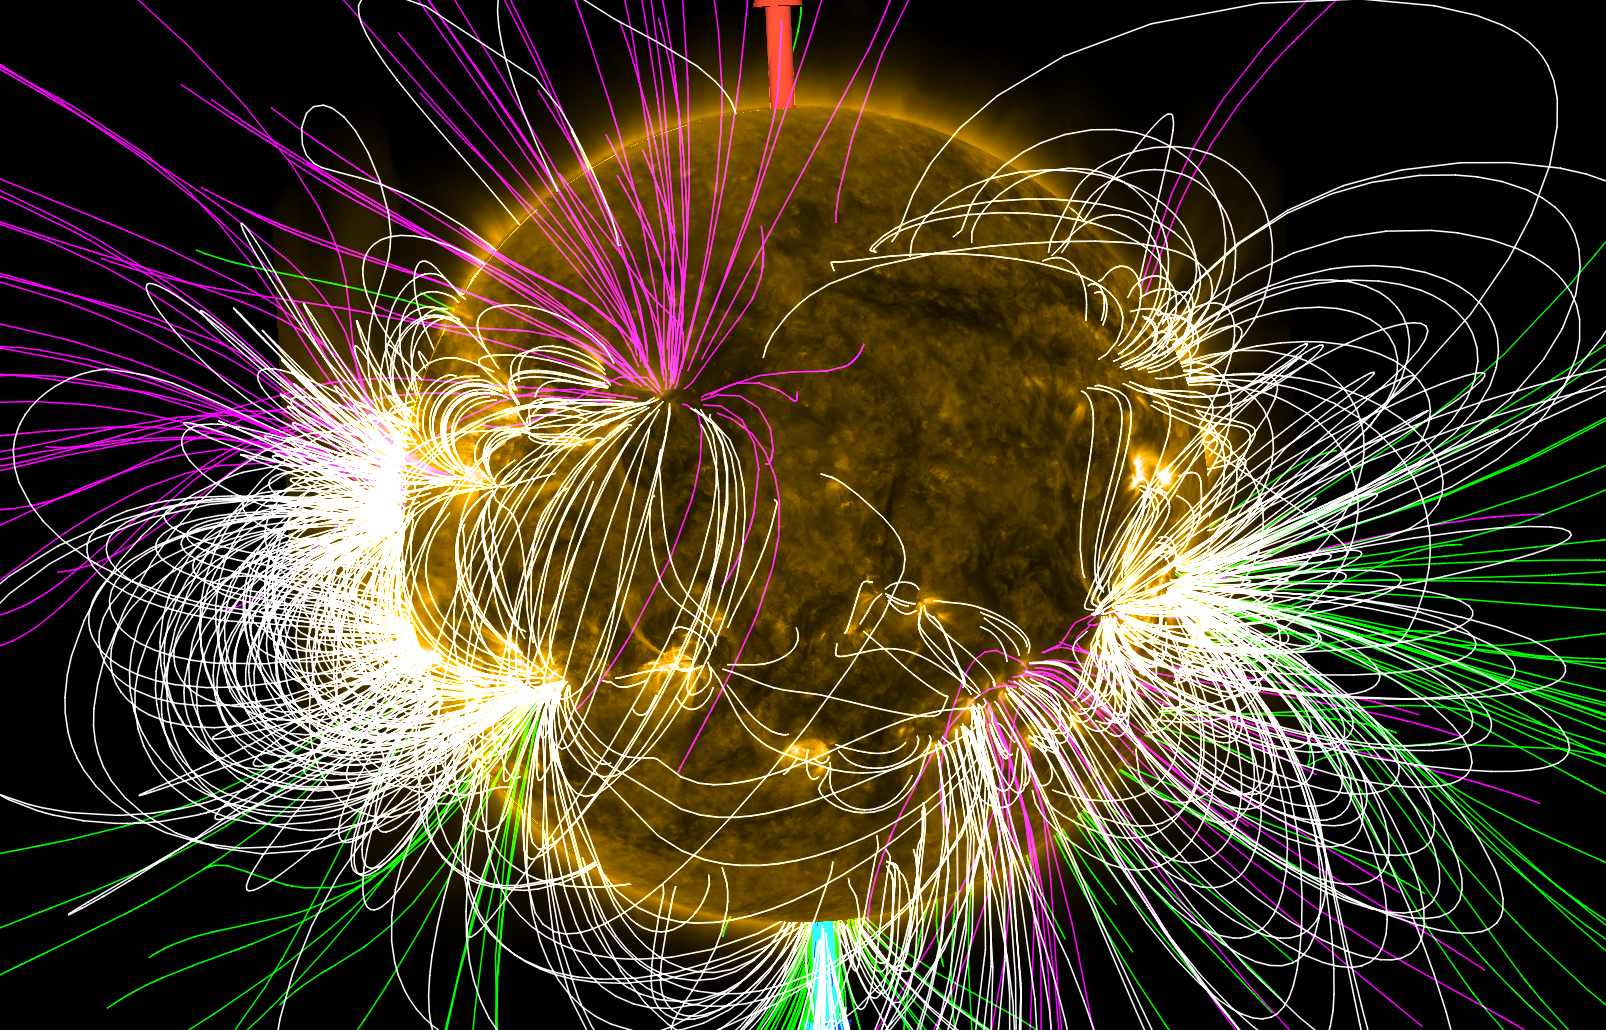
\includegraphics[width=13cm]{./pictures/title.png}\vspace{0.5cm}\\

\begin{onehalfspace}
\begin{huge}
\textbf{Feldlinien Kompression für JHelioviewer 3D}
\end{huge}
\vspace{0.1cm}\\
\begin{Large}
%\textbf{(Subtitle)}
\end{Large}
\vspace{0.8cm}\\
\begin{large}
\emph{Bachelorthesis von}\\
\textsc{Schwammberger}, Jonas\vspace{0.8cm}\\
FHNW\\
Hochschule für Technik\\
Studiengang Informatik\vspace{0.8cm}\\
\emph{Betreuer:}\\
\textsc{Csillaghy}, André\\
\textsc{Felix}, Simon\vspace{0.8cm}\\
\end{large}
\end{onehalfspace}
\vfill
\begin{normalsize}
Windisch, \today
\end{normalsize}
\pagebreak
\newpage

\pagestyle{abstract}
\section*{Abstract}
Ziel dieser Arbeit ist es eine verlustbehaftete Kompression für Feldlinien zu entwickeln, welche die Übertragung und das Caching im Arbeitsspeicher ermöglicht. In dieser Arbeit wurden drei Verfahren entwickelt: eine Kompression mit Adaptivem Subsampling, eine Kompression mit einer Diskreten Kosinus Transformation und eine Kompression mit Prädiktoren. Die höchste Kompressionsrate wurde mit der Diskreteten Kosinus Transformation erreicht, während die Kompression mit Adaptiven Subsamplings minimale Kompressionsartefakte aufweist. Die Kompression mit Prädiktoren ist ein Kompromiss zwischen Kompressionsrate und Artefakte.

Die Übertragung und Zwischenspeicherung von Feldlinien ist mit den entwickelten Verfahren möglich. Der Limitierende Faktor für die Kompression ist die Artefaktbildung: Ringing oder Ringing-Ähnliche Artefakte sind in Visualisierungen der Feldlinien störend. Wenn die Visualisierung ein Heranzoomen erlaubt, sind auch schwach ausgeprägte Artefakte zu erkennen. Eine höhere Kompressionsrate ist mit Verfahren zu erreichen, welche kaum oder keine Ringing Artefakte produzieren wie Wavelet Transformation, Curve Fitting oder Compressive Sensing.

\newpage
% Inhaltsverzeichnis
\pagestyle{tableofcontent}
\pagenumbering{Roman}
\tableofcontents  	
\newpage
\pagestyle{documentstyle}
\setcounter{page}{1}
\pagenumbering{arabic}

\section{Verwendung und Umfeld des JHelioviewers}
Wie der Name bereits verrät ist JHelioviewer eine Applikation,  die zur Analyse von Sonnendaten verwendet wird. Es wird international zur Sonnenforschung eingesetzt und wird von der FHNW zusammen mit der ESA entwickelt. Momentan ist eine neue Version des JHelioviewer in Entwicklung, welche die Sonne im dreidimensionalen Raum darstellt. Ein Feature von JHelioviewer ist die Magnetfeldlinien darzustellen und zu animieren, die Abbildung \ref{einleitung::feldlinien} zeigt die Visualisierung.
\begin{figure}[!htbp]
\center
	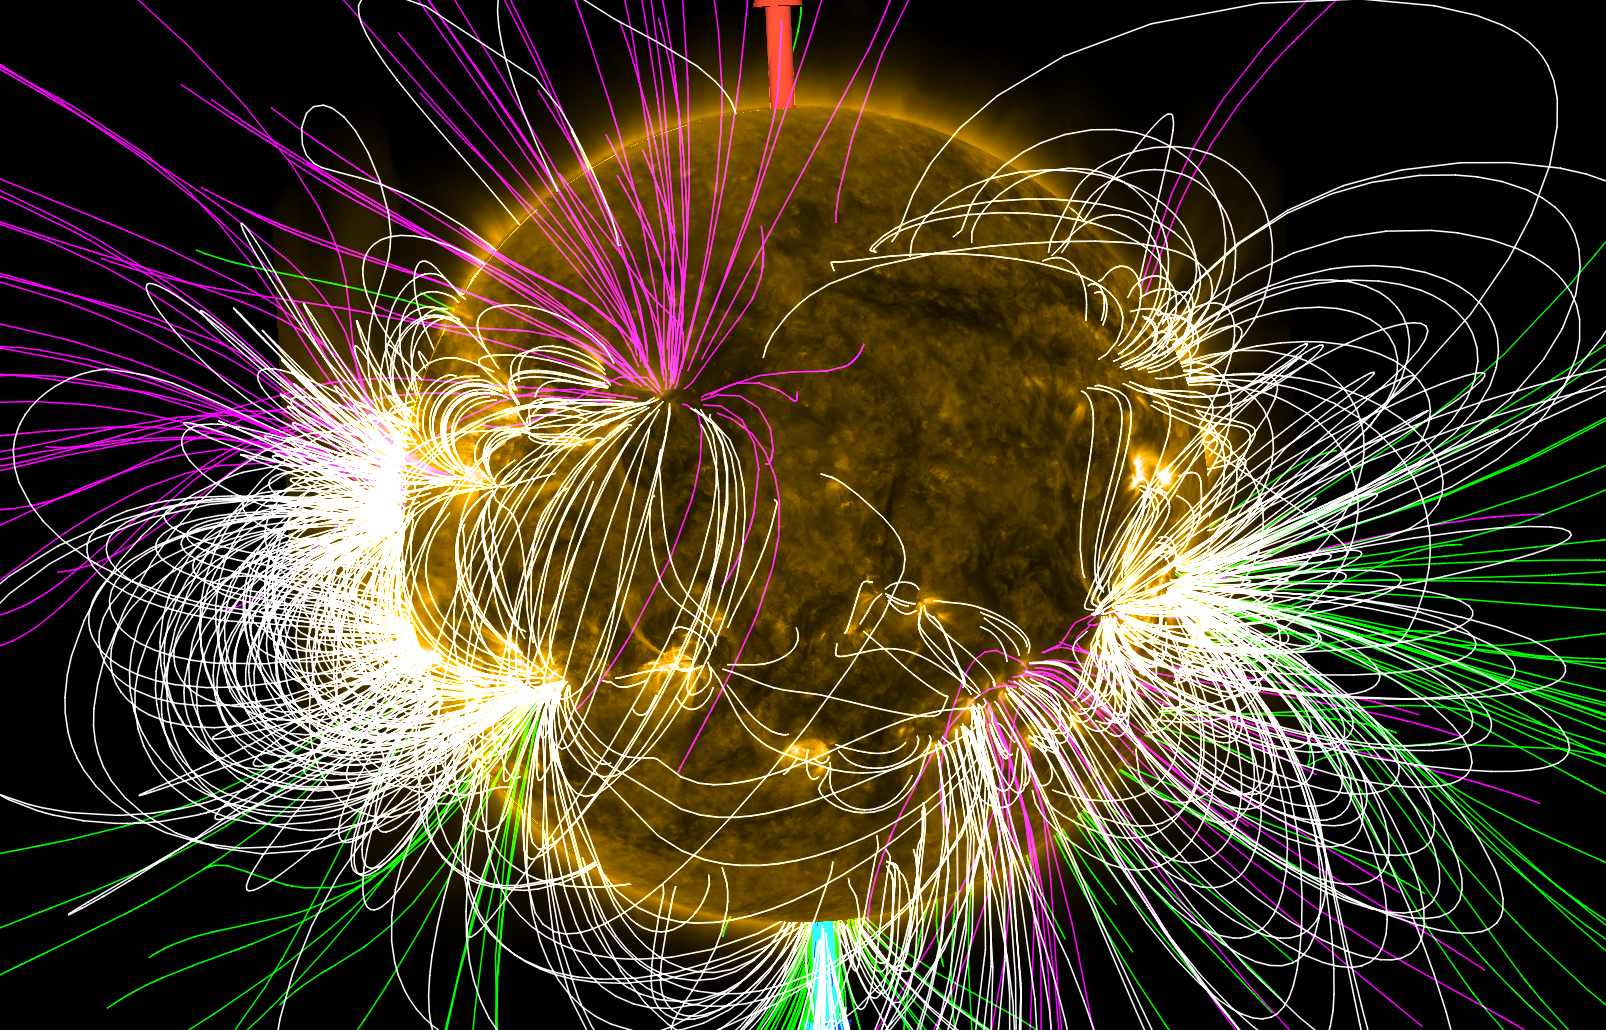
\includegraphics[scale=0.5]{./pictures/einleitung/fieldLines.png}
	\caption{Visualisierung der Feldlinien im JHelioviewer}
	\label{einleitung::feldlinien}
\end{figure}
Es wird zwischen drei Feldlinien Unterschieden: Linien, die auf der Sonne starten und wieder auf der Sonne landen, auf der Sonne starten und ins Weltall führen oder vom Weltall auf der Sonne landen. Die weissen Feldlinien repräsentieren ''Sonne zu Sonne´´, die Grünen ''Sonne zu Weltall´´ und die Violetten ''Weltall zu Sonne´´. Die Feldlinien sind, allgemein Betrachtet, eine grosse Menge an Punkten, welche ein Server bereitstellt. Die Abbildung \ref{einleitung::aufbau} visualisiert den Datenfluss.
\begin{figure}[!htbp]
\center
	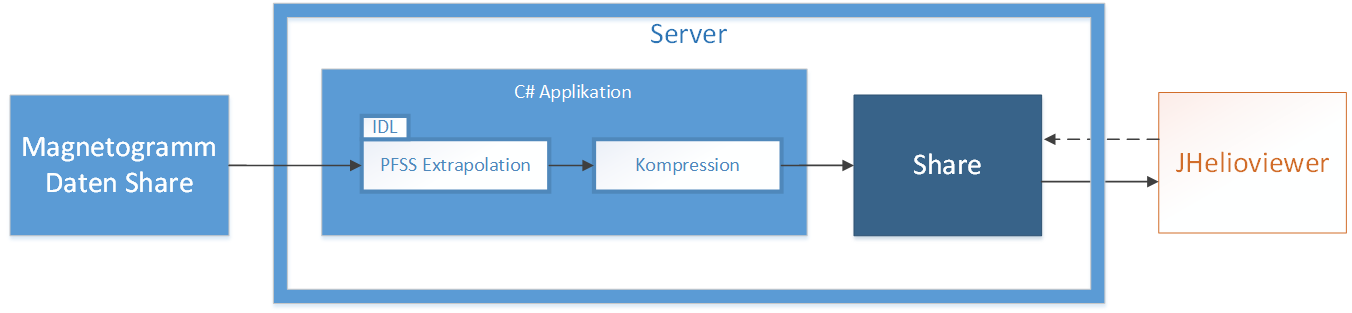
\includegraphics[scale=0.5]{./pictures/einleitung/server.png}
	\caption{Aufbau und Datenfluss des Servers}
	\label{einleitung::aufbau}
\end{figure}
In regelmässigen Abständen sucht der Server nach neuen Oberflächen-Magnetogramm-Daten der Satelliten. Alle sechs Stunden wird die Oberfläche der Sonne neu gemessen.Daraus werden mittels Potential Field Source Surface (PFSS) Extrapolation die Feldlinien zu diesem Zeitpunkt errechnet. Danach führt der Server eine verlustlose Kompression durch und stellt die Daten auf einem öffentlichen Share dem JHelioviewer zur Verfügung. Der JHelioviewer lädt dann zur Laufzeit die Feldlinien, die er benötigt. 

Zukunft soll eine Feldlinienanimation angeboten werden, nicht nur alle 6 stunden sondern jede halbe Stunde.

\subsection{Datenmenge ist zu gross für die Datenübertragung}
Die Feldlinien der Sonne zu einem Zeitpunkt bringen etwa 1.3 MiBytes auf die Waage. 

Mit einer vernünftigen Bandbreite ist das flüssige Abspielen der Animation deshalb nicht möglich. Ziel ist es eine Kompression zu entwickeln, welche eine flüssige Animation erlaubt.\\[\baselineskip]
Im Vorfeld möglichst verlustfrei
Neu verlustbehaftet

Ziel ist es die Feldlinien verlustbehaftet zu komprimieren, sodass JHelioviewer eine möglichst flüsssige Animation anbieten kann. Die Komprimierung soll serverseitig mittels C\# umgesetzt werden während der JHelioviewer mit der Dekomprimierung ausgestattet wird.\\[\baselineskip] 
Verlustbehaftet, metriken!!

 
\newpage
\section{State of the Art}
Die Teilschritte einer verlustbehaftete Kompressionen können in drei Verarbeitungsarten eingeteilt werden: Transformationen, Quantisierungen und Entropie Kodierungen. Die Abbildung \ref{state:aufbau} zeigt eine vereinfachte Abfolge. Die Inputdaten werden durch ein oder mehrere Verfahren transformiert. Die Transformationen haben das Ziel die Daten aufzubereiten, sodass die folgende Quantisierungen unwichtige Informationen löschen können. Die Transformationen sind  verlustfrei umkehrbar, in den Quantisierungsschritten werden typischerweise Informationen gelöscht. Im letzten Verarbeitungsschritt werden reduzierte Information wird Entropie Kodiert. Die Entropie Kodierung versucht die Information mit einem Minimum an Daten abzubilden.n\\
\begin{figure}[!htbp]
	\center
	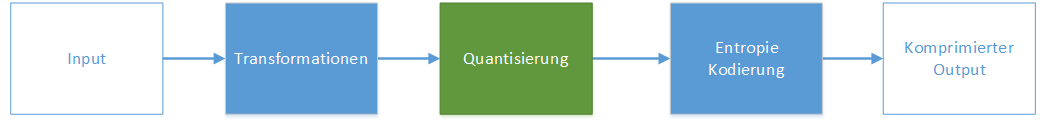
\includegraphics[width=0.8\textwidth,height=6cm,keepaspectratio]{./pictures/state/aufbau.png}
	\caption{Vereinfachter Ablauf einer verlustbehafteten Kompression}
	\label{state:aufbau}
\end{figure}

\subsection{JPEG/JFIF Bildkompression}
\begin{figure}[!htbp]
	\center
	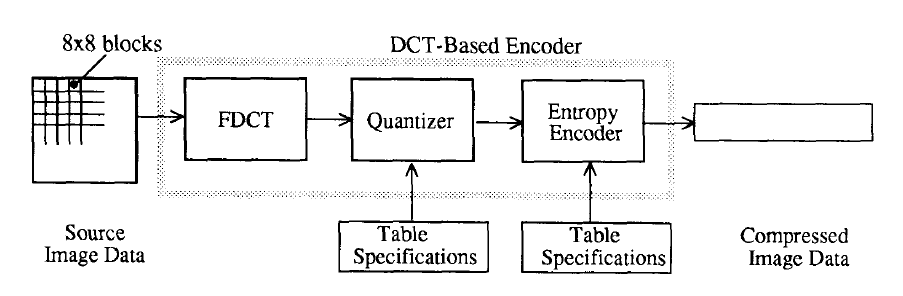
\includegraphics[width=0.8\textwidth,height=6cm,keepaspectratio]{./pictures/state/jpeg.png}
	\caption{Aufbau der JPEG Kompression \cite{wallace1992jpeg}}
	\label{state:jpeg:abb}
\end{figure}
Der JPEG/JFIF Standard ist eines der meist verwendeten Bildkompressionsalgorithmen für natürliche Bilder. Das Diagramm der Abbildung \ref{state:jpeg:abb} zeigt den Aufbau der Kompressionspipeline. JPEG/JFIF unterteilt das Eingabebild in $8*8$ Blöcke und führt eine Diskrete Kosinus Transformation (DCT) durch. Der Bildblock ist als Folge von Kosinus Funktionen dargestellt.\\
Die Quantisierung versucht Frequenzen, welche das menschliche Auge schlecht erkennen kann, zu quantisieren und mit weniger Präzision darzustellen. Wenn die Quantisierung gut gewählt wurde, kann das menschliche Auge das dekomprimierte Bild nicht vom Original unterscheiden. JPEG/JFIF bietet vorgefertigte Quantisierungstabellen an. Der Benutzer kann aber auf den anwendungsfall spezialisierte Tabellen anwenden. Wie die Quantisierungstabelle optimal gewählt wird, ist ein aktives Forschungsfeld \cite{wu1993rate:jpeg} \cite{wang2001designing:jpeg} und kann von Anwendungsfall zu Anwendungsfall unterschiedlich sein.\\
Nach der Quantisierung werden die quantisierten Blöcke im Zick-Zack-Muster angeordnet, sodass die Entropie Kodierung eine bessere Kompression durchführen kann. JPEG/JFIF führt eine Run-Length\cite{wiki:rle} und eine Huffman-Kodierung\cite{huffman1952method} durch. JPEG bietet auch hier an, eine benutzerspezifizierte Huffman-Tabelle zu verwenden.

Wenn für die Kompression von wissenschaftlichen Daten eine Diskrete Kosinus Transformation eingesetzt wird, kann ein ähnlicher Aufbau verwendet werden wie der JPEG/JFIF Standard. Für eine optimale Kompression wird die Umsetzung der einzelnen Schritte vom Standard abweichen.

\subsection{Point Cloud Kompression} \label{state:pointcloud}
\begin{figure}[!htbp]
	\center
	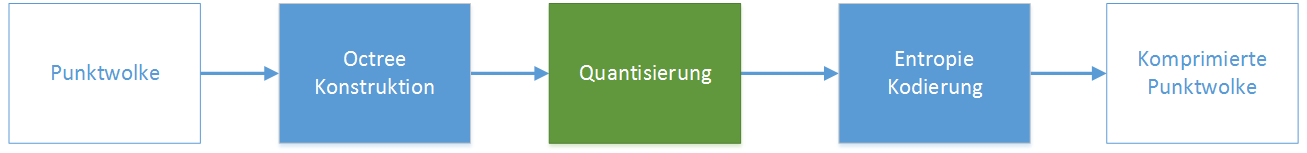
\includegraphics[width=0.8\textwidth,height=6cm,keepaspectratio]{./pictures/state/pointcloud.png}
	\caption{Aufbau einer Octree basierten Point Cloud Kompression.}
	\label{state:pointcloud:abb}
\end{figure}
3d Laser Sampling Geräte produzieren grosse Mengen an dreidimensionalen Punkten von alltäglichen Objekten. Die Kompression von solchen Punktwolken ist ein aktives Forschungsfeld. Eine vorgeschlagene Kompression  von Schnabel und Klein \cite{schnabel2006octree} verwendet Octrees \cite{wiki:octree}. Das Diagramm der Abbildung \ref{state:pointcloud:abb} verdeutlicht den Ablauf.\\
Die dreidimensionalen Punkten werden in einem Octree mit einer begrenzten Anzahl an Levels abgelegt. Im Quantisierungsschritt werden die Punkte durch die Zellenmittelpunkte des Octrees ersetzt. Die Anzahl an Levels ist gleichzusetzen mit der Genauigkeit in Bits welche für jede Koordinatenachse zur Verfügung stehen. Wenn die Levels auf $8$ begrenzt sind, steht für jede Achse $8$ Bit Genauigkeit zur Verfügung.\\
In der Entropie Kodierung wird der Octree in Breadth-First Ordnung binär abgebildet ($0$ für leere Knoten, $1$ für befüllte Knoten). Jedes Level im Octree repräsentiert eine Approximation der Punktwolke. Durch  die Breath-First Ordnung werden die ungenaueren Approximationen zuerst abgelegt. Diese Eigenschaft wird mit einer Prediktiven Kodierung ausgenutzt: Aus den vorhergehenden Levels wird die Punktverteilung des nächsten Level vorhergesagt. Die Kodierung kann die Information reduzieren, indem nur noch der Fehler der Vorhersage abgespeichert wird.

Um die Point Cloud Kompression auf die Feldlinien anzuwenden muss die Information gespeichert werden, welcher Punkt zu welcher Linie gehört. Schnabel und Klein stellen einen angepassten Algorithmus vor, welcher eine Punktwolke mit Farbinformationen komprimiert. Die Farbinformation kann verwendet werden um einen Punkt einer Feldlinie zuzuordnen. Weiter muss die Prediktive Kodierung angepasst werden: Schnabel und Klein nehmen an, dass die Punktwolke eine Oberfläche darstellen. Die Feldlinien bilden im Allgemeinen keine Oberfläche und benötigen deshalb eine andere Prediktive Kodierung.

\subsection{Curve Fitting}
Curve Fitting ist ein Prozess, welcher ein Signal durch eine oder mehrere Funktionen abbildet. Es ist zwischen einem exakten Curve Fitting und einer Approximation zu unterscheiden. Die exakte Repräsentation wird typischerweise für die Signalinterpolation und eine Approximation in der Rauschunterdrückung verwendet. Eine Datenkompression ist mit Curve Fitting möglich, wenn die Parameter der approximierenden Funktionen weniger Speicherplatz benötigen, als das Signal.\\
Unser et al \cite{unser1993b:spline} zeigt ein Algorithmus, welcher ein diskretes Signal als Folge von B-Splines darstellt. Unser stellt ein mögliches Verfahren für verlustbehaftete Bildkompression mittels B-Splines vor\cite{unser1993b2:spline}. Der Vorteil der B-Splines ist, dass die Artefakte der Dekompression als Rauschunterdrückung und Schärfung des Originalbildes ausdrücken.

Eine Datenkompression mit Curve Fitting ist im Vergleich mit der Kosinus Transformation weniger erforscht. Es sind ebenfalls keine Kompressionsstandards bekannt, welche ein Curve Fitting für die Datenkompression verwenden. Ein Kompressionsverfahren zu entwickeln zieht zusätzlichen Aufwand mit sich als Verfahren, welche in der Datenkompression etabliert sind.

\subsection{Compressive Sensing}
Compressive Sensing ist ein Verfahren, welches ein Signal mit einer minimalen Anzahl an Funktionen aus einem Dictionary darstellt (sparse representation).  Die Funktionen im Dictionary sind durch keine Rahmenbedingungen begrenzt, jede allgemeine Funktion im Dictionary des Compressive Sensing verwendet werden. 

Das Überführen in die sparse representation ist ein $np-hard$ Problem \cite{wiki:npHard}. Es existieren aber Heurisiken wie Orthogonal Matching Pursuit\cite{tropp2007signal}, welches in linearer Laufzeit eine approximation erstellt. Die Approximation ist für jeden Anwendungsfall genügend genau.

Mit einem allgemeinen Dictionary ist jedes Signal rekonstruierbar. Die Stärke des Compressive Sensing Ansatzes ist, dass das Dictionary auf die Signale optimiert werden kann. Ein möglicher Algorithmus ist der K-SVD \cite{bryt2008compression} Algorithmus. K-SVD ist ein Unsupervised Learning Algorithmus und erlernt ein Dictionary anhand von Beispielsignalen.

Compressive Sensing hat das Potential eine hohe Kompressionsrate zu erreichen. Die Feldlinien sind oft ähnlich und unterscheiden sich hauptsächlich in Rotation, Verschiebung und Skalierung. Mit einem auf Feldlinien angepasstes Dictionary kann eine Feldlinie durch wenige Funktionen approximiert werden.

\subsection{Entropie Kodierung}
Die Entropie Kodierung findet in allen Bereichen der Informatik Anwendungen. Ziel ist es die gleiche Information mit einem Minimum an Daten darzustellen. Verlustbehaftete Kompressionsverfahren reduzieren die Information und verwenden im letzten Schritt eine Entropie Kodierung um die Datenmenge zu reduzieren.

Es ist zwischen spezialisierten und allgemeinen Entropie Kodierer zu unterscheiden. Unter den spezialisierten Verfahren ist Beispielswiese die Arbeit von Ratanaworabhan et al.\cite{ratanaworabhan2006fast} einzuordnern, welche in der Lage ist Floating Point Daten performant zu kodieren und dekodieren.
 
Unter den allgemeinen Verfahren sind Archivierer wie GZIP\cite{website:gzip}, 7-ZIP\cite{website:7zip} und RAR\cite{website:rar} angesiedelt. Archivierungsverfahren finden in allen Bereichen Anwendung und dienen in der Entwicklung von spezialisierten Kodierer als Messbasis. Im Vorfeld wurde die Kompressionsraten von GZIP, 7-ZIP und RAR von Feldliniendaten verglichen, wobei RAR die höchsten Raten erreichen konnte.\\
GZIP und 7-ZIP bestehen aus einer Kombination von Entropie Kodierer. RAR hingegen besitzt unterschiedliche Kombinationen und wählt das Verfahren aus, welches die Input Daten optimal kodieren kann. Dadurch kann RAR für unterschiedliche Daten eine hohe Kompressionsrate erreichen. Die RAR Kompression ist urheberrechtlich Geschützt und die verwendeten Algorithmen sind nicht bekannt.
\newpage
\section{Kompressionsverfahren der Feldlinien} \label{konzept}
In diesem Abschnitt werden die einzelnen Verfahren zu den Lösungsansätzen vorgestellt. Im ersten Abschnitt \ref{konzept:ist-komprimierung} wird die Ist-Kompression analysiert, während in den nächsten Abschnitten die  Lösungsansätze vorgestellt werden und die Teilschritte erklärt.

\subsection{Ist-Komprimierung} \label{konzept:ist-komprimierung}
\begin{figure}[!htbp]
	\center
	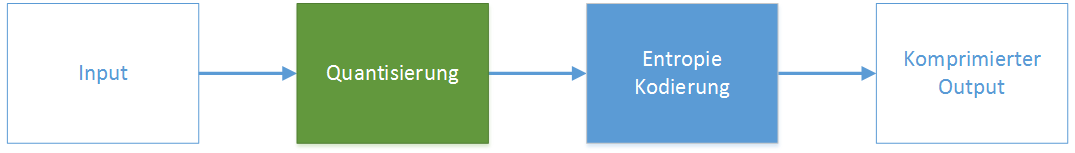
\includegraphics[width=0.8\textwidth,height=6cm,keepaspectratio]{./pictures/konzept/ist/aufbau.png}
	\caption{Aufbau der Ist-Kompression.}
	\label{konzept:ist:aufbau:diagramm}
\end{figure}
Das Ziel der Ist-Kompression ist es, die Datenmenge mit einfachen Mitteln drastisch zu reduzieren. Der Aufbau ist im Diagramm der Abbildung \ref{konzept:ist:aufbau:diagramm} dargestellt. Die Ist-Kompression führt zuerst ein Subsampling durch. Drei Viertel aller Punkte werden in diesem Schritt verworfen. Im nächsten Schritt werden die übrigen Punkte  auf 16-Bit Integer diskretisiert. Das reduziert die Anzahl Bytes und verbessert die Kompression im Schritt Entropie Kodierung. Die Implementationen der Entropie Kodierer scheinen Integer-Werte einfacher komprimieren zu können. In der Entropie Kodierung werden die Daten geordnet wie in Tabelle \ref{konzept:ist:entropie} dargestellt.
\begin{table}[!htbp]
	\center
	\begin{tabular}{|c|c|c|c|}
	\hline
	Anzahl Punkte der Feldlinien & X Kanal aller Punkte & Y Kanal aller Punkte & Z Kanal aller Punkte \\\hline
	\end{tabular}
	\caption{Anordnung der Simulationsdaten der Ist-Kompression}
	\label{konzept:ist:entropie}
\end{table}
Als erstes werden die Längen aller Feldlinien abgelegt. Danach folgt der X, Y und der Z Kanal aller Punkte der Feldlinien. Diese Anordnung verbessert die Kompressionsrate der Entropie Kodierung. Je näher ähnliche Muster beieinander liegen, desto besser können sie Komprimiert werden. Für die eigentliche Entropie-Kodierung wird Gzip verwendet. Gzip basiert auf dem Deflate Algorithmus, welcher aus einer Kombination von LZ77 und Huffman Kodierung besteht \cite{wiki:gzip}.\\
Die Punktmenge ist für Low-End Grafikkarten zu gross. Um die Punktmenge für die Visualisierung zu verkleinern, führt der JHelioviewer ein weiteres Subsampling durch, welches im Abschnitt \ref{konzept:loesung0:subsampling} beschrieben ist.

\subsection{Lösungsansatz: Adaptives Subsampling} \label{konzept:loesung0}
\begin{figure}[!htbp]
	\center
	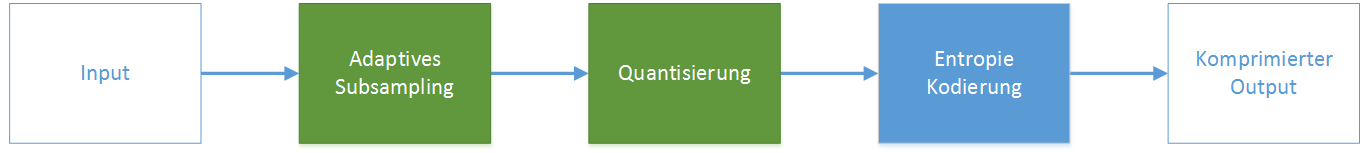
\includegraphics[width=0.8\textwidth,height=6cm,keepaspectratio]{./pictures/konzept/solution0/aufbau.png}
	\caption{Aufbau des Lösungsansatzes: Adaptives Subsampling.}
	\label{konzept:loesung0:aufbau:diagramm}
\end{figure} 
Dieser Lösungsansatz verwendet einen ähnlichen Aufbau wie die Ist-Kompression \ref{konzept:ist-komprimierung}. Der Unterschied ist, dass das Subsampling Verfahren gewählt wurde, welches der JHelioviewer auf dem Client durchführt. Die Abbildung \ref{konzept:loesung0:aufbau:diagramm} zeigt den neuen Ablauf.\\
Dieser Ansatz überträgt nur die Information, die der JHelioviewer zur Visualisierung benötigt. Der Vorteil ist dass die Information, die der JHelioviewer visualisiert ein Bruchteil darstellt und somit eine hohe Kompressionsrate ereicht werden kann. Es ist möglich dass die Visualisierung zu einem späteren Zeitpunkt mehr Punkte darstellen soll. In diesem Fall müssten entweder mehr Punkte übertragen werden, was eine schlechtere Kompressionsrate zur Folge hat, oder der JHelioviewer muss eine Interpolation durchführen. 

\subsubsection{Adaptives Subsampling}\label{konzept:loesung0:subsampling}
Konzeptionell approximiert das adaptive Subsambling eine Kurve diruch eine Folge von Strecken. Je stärker die Krümmung der Kurve, desto mehr Strecken werden für die Approximation benötigt.
\begin{figure}[!htbp]
	\center
	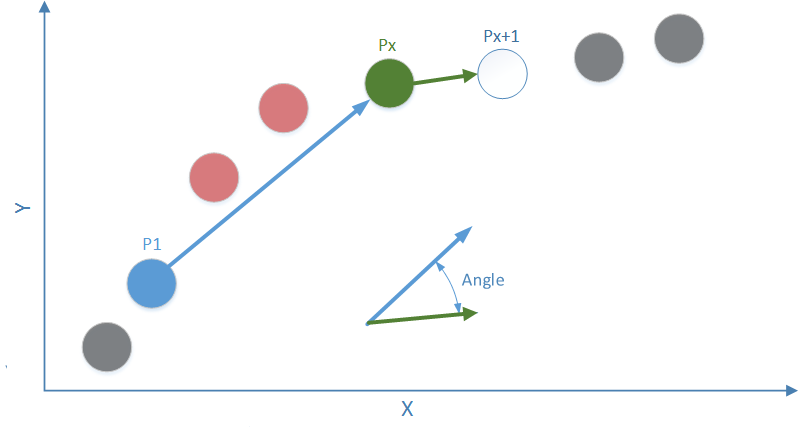
\includegraphics[width=0.8\textwidth,height=6cm,keepaspectratio]{./pictures/konzept/solution0/anglesubsampling.png}
	\caption{Darstellung des Adaptiven Subsapmlings im 2D Raum. Rot sind die Punkte, welche geprüft und gelöscht wurden. Grün ist der Punkt dargestellt, welcher geprüft wird.}
	\label{konzept:loesung0:angle}
\end{figure}
Das Diagramm der Abbildung \ref{konzept:loesung0:angle} stellt das Subsampling im zweidimensionalen Raum dar. Das Adaptive Subsampling wählt nun Punkte $P$ aus der Feldlinie aus, welche Start- und Endpunkte der Strecken darstellen.\\
$P_1$ wurde bereits ausgewählt. Es wird nun ein Punkt $P_x$ gesucht, der als Endpunkt einer Strecke von $P_1$ zu $P_x$ die Feldlinie approximiert. Dazu wird der Winkel der Strecke $P_1$ zu $P_x$ mit der Strecke $P_x$ zu $P_x+1$ verglichen. Wenn der Winkel kleiner ist, als ein Winkel $\alpha$, wird der nächste Punkt $P_x+1$ überprüft. Wenn der Winkel grösser ist, wird $P_x$ ausgewählt. Danach wird der wird eine nächste Strecke startend von $P_x$ gesucht.

\subsubsection{Entropie Kodierung mittels RAR} \label{konzept:loesung0:kodierung}
Die Anordnung der Daten wurde aus der Ist-Kompression übernommen, jedoch wird Rar anstatt GZip verwendet. GZip konnte bei den Ist-Komprimierten Daten eine Kompressionsrate von $1.2$ erreichen, während Rar bei selben Daten eine Rate von $3.7$ erreicht.
\pagebreak

\subsection{Lösungsantz: Diskrete Kosinus Transformation}\label{konzept:loesung1}
\begin{figure}[!htbp]
	\center
	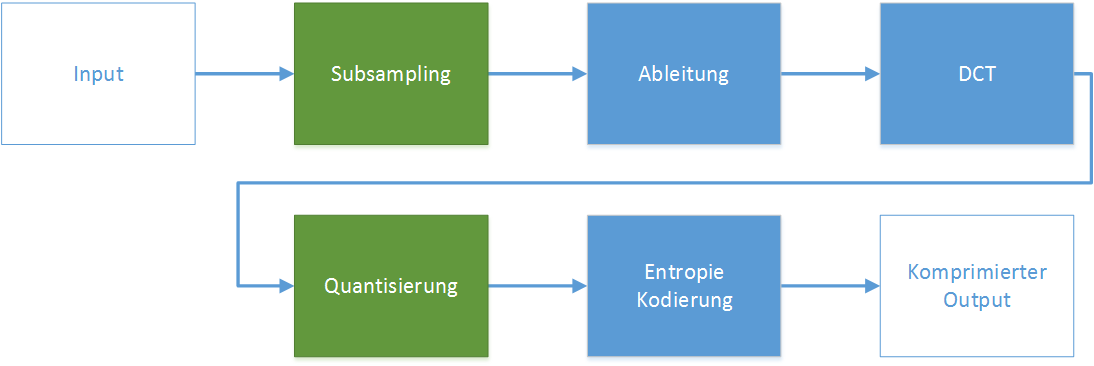
\includegraphics[width=0.8\textwidth,height=6cm,keepaspectratio]{./pictures/konzept/solution1/aufbau.png}
	\caption{Aufbau des Lösungsansatzes: Adaptives Subsampling.}
	\label{konzept:loesung1:aufbau}
\end{figure} 
Die Kompression dieses Lösungsansatzes ist Dargestellt im Diagramm der Abbildung \ref{konzept:loesung1:aufbau}. Konzeptionell ähnelt dieser Ansatz der JPEG/JFIF Kompression (dargestellt in der Abbildung \ref{state:jpeg:abb}), die einzelnen Teilschritte können aber andere Algorithmen verwenden. Im Vergleich zum JPEG/JFIF Standard ist der grösste Unterschied, dass das Eingangssignal vor der Kosinus Transformation abgeleitet wird.

Die Feldlinien ähneln oft harmonischen Halbwellen, welche sich durch wenige Kosinusfunktionen approximieren lassen können. Um eine optimale Kompression mit dieser Variante zu erreichen, müssen Ringing Artefakte \cite{wiki:ringing:artefacts} behandelt werden. Sie äussern sich als Oszillieren im dekomprimierten Signal, was das menschliche Auge als störend empfindet. Beispiele für die Ringing Artefakten von Feldlinien sind im Abschnitt \ref{resultate:loesung1:ringing} zu finden.\\
Es gibt Möglichkeiten, die Ringing Artefakte zu Dämpfen oder gar zu beheben: Die simpelste Variante ist es, das dekomprimierte Signal zu glätten. Die Glättung kann das Signal verfälschen und ist deshalb nicht die optimale Lösung. In der Bild- und Audioverarbeitung wird aktiv nach Post-Processing Filter geforscht, welche die Ringing Artefakte in der Dekompression vermindern \cite{kaup1998reduction} \cite{park1999postprocessing}. Ein angepasstes Postprocessing wurde im Rahmen dieser Arbeit nicht implementiert.

\subsubsection{Subsampling} \label{konzept:loesung1:subsampling}
Das Subsampling wurde aus der Ist-Kompression \ref{konzept:ist-komprimierung} übernommen und dient, die DCT zu beschleunigen. Da die DCT eine Komplexität von $O(n^2)$ aufweist, wird durch das Subsampling die Transformation wesentlich beschlenuitgt.\\
Falls die Laufzeit der Dekompression weiter verbessert werden soll, kann die Fast-Cosine-Transformation umgesetzt werden. Diese hat eine Komplexität von $O(n log(n))$. Falls das nicht ausreicht, können die Linien in Blöcke unterteilt werden und die DCT pro Block ausführen. Dadurch wird die Komplexität auf $O(n)$ gesenkt. Jedoch ist es wahrscheinlich, dass durch die Unterteilung die Kompressionsrate leidet. Die Approximation mehrer Blöcke des Eingabesignals benötigt schlussendlich mehr Kosinusfunktionen, als die Approximation des gesamten Signals.

\subsubsection{Ableitung}
Das Eingabesignal wird abgeleitet und alle folgenden Transformationen werden auf den Steigungen des Signals ausgeführt. Damit die Transformation umkehrbar ist, muss der Startpunkt zusätzlich abgespeichert werden.\\
Die Artefakte, welche das abgeleitete dekomprimierte Signal beinhaltet, sind bei der Feldliniensimulation weniger störend für das menschliche Auge. Die Feldlinie bleibt tendenziell glatt und Artefakte äussern sich meist in veränderten Amplituden, welche erst erkennbar sind, wenn die Originalfeldlinie zum Vergleich bereit steht. Diese Eigenschaft wirkt sich ebenfalls auf die Ringing-Artefakte aus. Die Ableitung hat einen dämpfenden Effekt auf die Ringing Artefakte.

\subsubsection{Cosinus-Transformation} \label{konzept:loesung1:kosinus}
Die Diskrete Kosinus Transformation stellt eine endliche Menge von $N$ Datenpunkten als $N$ Kosinusfunktionen zu verschiedenen Frequenzen dar. Die Werte DCT-Koeffizienten stellt dar, wie hoch der Anteil einer bestimmten Frequenz ist im Originalsignal. Im optimalen Fall kann ein Signal durch niederfrequente Funktionen approximiert werden. Die hochfrequenten Anteile stellen Details dar, welche meist nicht relevant sind.\\
Es gibt verschiedene Möglichkeiten die Punkte zu transformieren. Hier wurde sich am JPEG/JFIF Standard orientiert, welche die DCT-II \eqref{konzept:loesung1:kosinus:formula:fdct} als Forwärts und die DCT-III \eqref{konzept:loesung1:kosinus:formula:idct} als Rückwärtstransformation verwendet \cite{wallace1992jpeg}. 
\begin{equation} \label{konzept:loesung1:kosinus:formula:fdct}
	X_k = \sum_{n=0}^{N-1}x_n*cos[\frac{\pi}{N}k(n+\frac{1}{2})] \quad k = 0, 1, \ldots, N-1
\end{equation}
\begin{equation} \label{konzept:loesung1:kosinus:formula:idct}
x_n  = \frac{1}{2}X_0 + \sum_{k=1}^{N-1}X_k*cos[\frac{\pi}{N}k(n+\frac{1}{2})] \quad n = 0,1,\ldots,N-1
\end{equation}
$N$ bezeichnet die Länge des Eingabesisignals, $x_n$ bezeichnet einen Wert im diskreten Signal und $X_k$ ist der Anteil der Frequens $k$. Ein Eingabesignal der Länge $N$ resultiert in $N$ Kosinus-Funktionen.

Die DCT transformiert ein periodisches, unendliches Signal. Um ein endliches Signal zu transformieren, wird es konzeptionell wiederholt. Die gewählten Verfahren wiederholen das Signal jeweils in umgekehrter Reihenfolge.\\
Die Wiederholung beeinflusst die Transformation nicht, wenn das Signal an den Rändern abflacht. Falls das Signal nicht abflacht, können nach der Quantisierung an den Rändern markante Artefakte auftreten. Ein Beispiel für solche Artefakte ist im Diagramm der Abbildung \ref{resultate:loesung1:dct:artefakte} im Abschnitt \ref{resultate:dct} zu sehen.

\subsubsection{Quantisierung}
In der Visualisierung werden die Feldlinien in drei Typen unterschieden: ''Sonne zu Sonne'', ''Sonne ins Weltall'' und ''Weltall zur Sonne''.  Die ''Sonne zu Sonne'' Feldlinien können besser durch Kosinusfunktionen approximiert werden und sind weniger Anfällig auf die Ringing Artefakte. Dieser Typ von Feldlinien wird deshalb stärker Quantisiert. Für die ''Sonne zu Sonne'' Feldlinien werden maximal $35$ DCT Koeffizienten abgelegt, wobei die letzten zehn Koeffizienten kaum noch Einfluss besitzen. Sie werden mit einem hohen Faktor quantisiert, sodass sie im Normalfall ebenfalls Null sind.\\
Die anderen Feldlinien benötigen mehr Koeffizienten für die Dämpfung der Ringing Artefakte. Bei ihnen liegt das Maximum bei $50$ Koeffizienten.

\subsubsection{Entropie Kodierung}\label{konzept:loesung1:kodierung}
Um die Entropie Kodierung zu verbessern wurden zwei Byte-Kodierungen hinzugefügt. Die Kanäle werden zuerst mit der Längenkodierung und darauf folgend mit der adaptive Genauigkeit kodiert.

\textbf{Längenkodierung}\\
Die Quantisierung erlaubt nur eine maximale Anzahl an Koeffizienten. Ab dem $50$ Koeffizient, sind die Werte Null. Die Längenkodierung schneidet den Block von Null-Koeffizienten ab und fügt die Länge des Nicht-Null Blockes hinzu. Alle Längen und alle Blöcke werden zusammen abgespeichert, die Tabelle \ref{konzept:loesung1:entropie:laengenkodierung} verdeutlicht das Konzept. $n_i$ ist die Länge der Feldlinie $i$ und $x_{i,j}$ ist der $j$ DCT-Koeffizient der Feldlinie $i$.\\
\begin{table}[!htbp]
	\center
	\begin{tabular}{||c|c|c|c|c||c|c|c}
		\hline
		\multicolumn{8}{|c|}{X Kanäle}\\\hline\hline
		 \multicolumn{5}{||c||}{Block Feldlinie 0} & \multicolumn{3}{c}{\ldots} \\\hline
		$n_0$ &$x_{0,0}$ &$x_{0,1}$ & \ldots & $x_{0,n-1}$ & $n_1$ & $x_{1,0}$ & \ldots\\\hline
	\end{tabular}
	\caption{Beispiel eines abgespeicherten Kanals mit der Längenkodierung.}
	\label{konzept:loesung1:entropie:laengenkodierung}
\end{table}
Um einen Kanal zu Dekodieren, muss die Anzahl an DCT-Koeffizienten $n_i$ gelesen werden und danach Nullen Anfügen, bis die ursprüngliche Länge des Kanals erreicht wurde. Die Anzahl Punkte jeder Feldlinie ist ebenfalls gespeichert.

Die Längenkodierung ist effizient, wenn die hochfrequenten DCT-Koeffizienten einen grossen, zusammenhängenden Null-Block bilden. Im schlechtesten Fall währe der letzte DCT-Koeffizient nicht Null. In diesem Fall würde die Längenkodierung nichts abschneiden.\\

\textbf{Adaptive Genauigkeits-Kodierung}\\
Die quantisierten Koeffizienten liegen meistens zwischen $-50$ und $+50$. Acht Bit Genauigkeit reichen im Allgemeinen aus um einen DCT-Koeffizienten abzuspeichern. Mit der adaptiven Genauigkeits-Kodierung sollen so wenige Bytes pro Koeffizient abgespeichert werden, wie benötigt werden. Dazu wird wie in Tabelle \ref{konzept:loesung1:entropie:adaptive} eine neue Byte-Kodierung eingeführt. Das MSB wird als ''Continue Flag'' verwendet. Wenn es gesetzt ist, gehört das folgende Byte ebenfalls zur Zahl.\\
\begin{table}[!htbp]
	\center
	\begin{tabular}{|c|c|c|c||c|c|c|c|}
	\hline
	\multicolumn{8}{|c|}{Byte}\\\hline
	Continue Flag & X & X & X & X & X & X & X \\\hline
	\end{tabular}
	\caption{Aufteilung eines Bytes der adaptiven Genauigkeitskodierung. X sind Nutz-Bits.}
	\label{konzept:loesung1:entropie:adaptive}
\end{table}
Wenn ein Kanal hauptsächlich aus tiefen Zahlen besteht, können so Bytes gespart werden, ohne Genauigkeit zu verlieren. Wenn aber der Kanal aus hauptsächlich grossen Zahlen besteht, welche zwei oder mehr Bytes an Genauigkeit brauchen, wird weniger Speicherplatz gespart.

\pagebreak
\subsection{Lösungsansatz: Prediktive Kodierung} \label{konzept:prediktiv}
\begin{figure}[!htbp]
	\center
	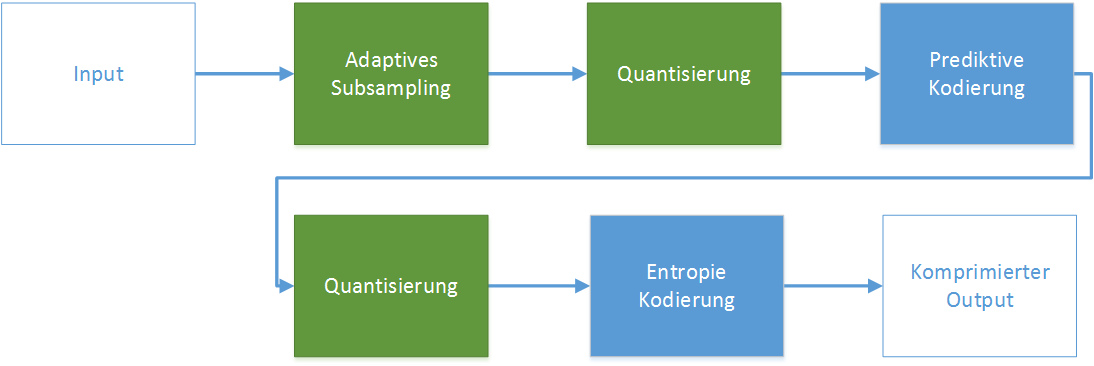
\includegraphics[width=0.8\textwidth,height=6cm,keepaspectratio]{./pictures/konzept/solution2/aufbau.png}
	\caption{Aufbau des Lösungsansatzes: Adaptives Subsampling.}
	\label{konzept:loesung2:aufbau}
\end{figure} 
Warum Prediktive Kodierung, was ist das gute: weniger sichtbare Artefakte, sie äussern sich hauptsächlich durch Verschiebungen. Prediktive Kodierung stammt aus der verlustfreien Kompression, wie also Daten gelöscht werden ist eine zentrale Frage.
Idee aus state of the art point cloud. Dort wird ein Octree verwendet, welche immer genauer die Daten approximiert.

\subsubsection{Angle Subsampling}
selbe subsampling wie lösung zuvor. es werden aber mehr punkte übertragen. Grund liegt darin dass das angle subsampling eine gute heuristik darstellt, unwichtige Informationen zu löschen.

\subsubsection{Quantisierung}
quantisierung in diskretisierten spärischen koordinaten. selbe wie in Lösung 0 aber angepasst?

\subsubsection{Wavelet Prediktive Kodierung}
 Das selbe Prinzip wird nun auf die Kurven der Kanäle übertragen werden. Kurven dar (ref pca der resultate).
Im Diagramm der Abbildung \ref{konzept:loesung2:algorithm:step1} ist der erste Schritt des Algorithmus dargestellt. Start und Endpunkt werden ohne Kodierung abgespeichert. Es wird der mittlere Punkt des Kanals kodiert. Es wird angenommen, dass der mittlere Punkt des Signals auf der Linie zwischen Start- und Endpunkt liegt.
Algorithmus Schritt 1: Residual
\begin{figure}[!htbp]
	\center
	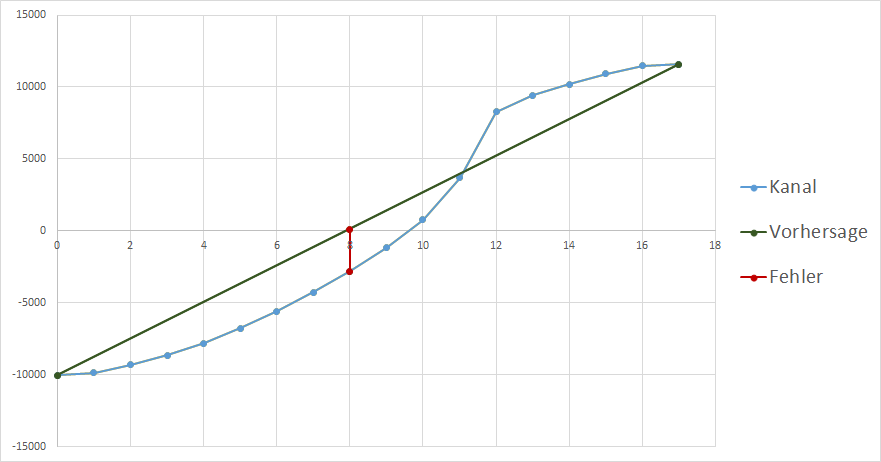
\includegraphics[width=1\textwidth,height=6cm,keepaspectratio]{./pictures/konzept/solution2/algorithm_step1.png}
	\caption{Erster Schritt der Wavelet Prediktiven Kodierung. Zu sehen sind das zu kodierende Signal, die Vorhersage und den Fehler der Vorhersage.}
	\label{konzept:loesung2:algorithm:step1}
\end{figure} 
Fehler von der Vorhersage zum Mittelpunkt. Nächster Schritt ist nun das ganze rekursiv für die neuen Teilstrecken zu wiederholen. Der nächste Schritt ist im Diagramm \ref{konzept:loesung2:algorithm:step2} dargestellt.
\begin{figure}[!htbp]
	\center
	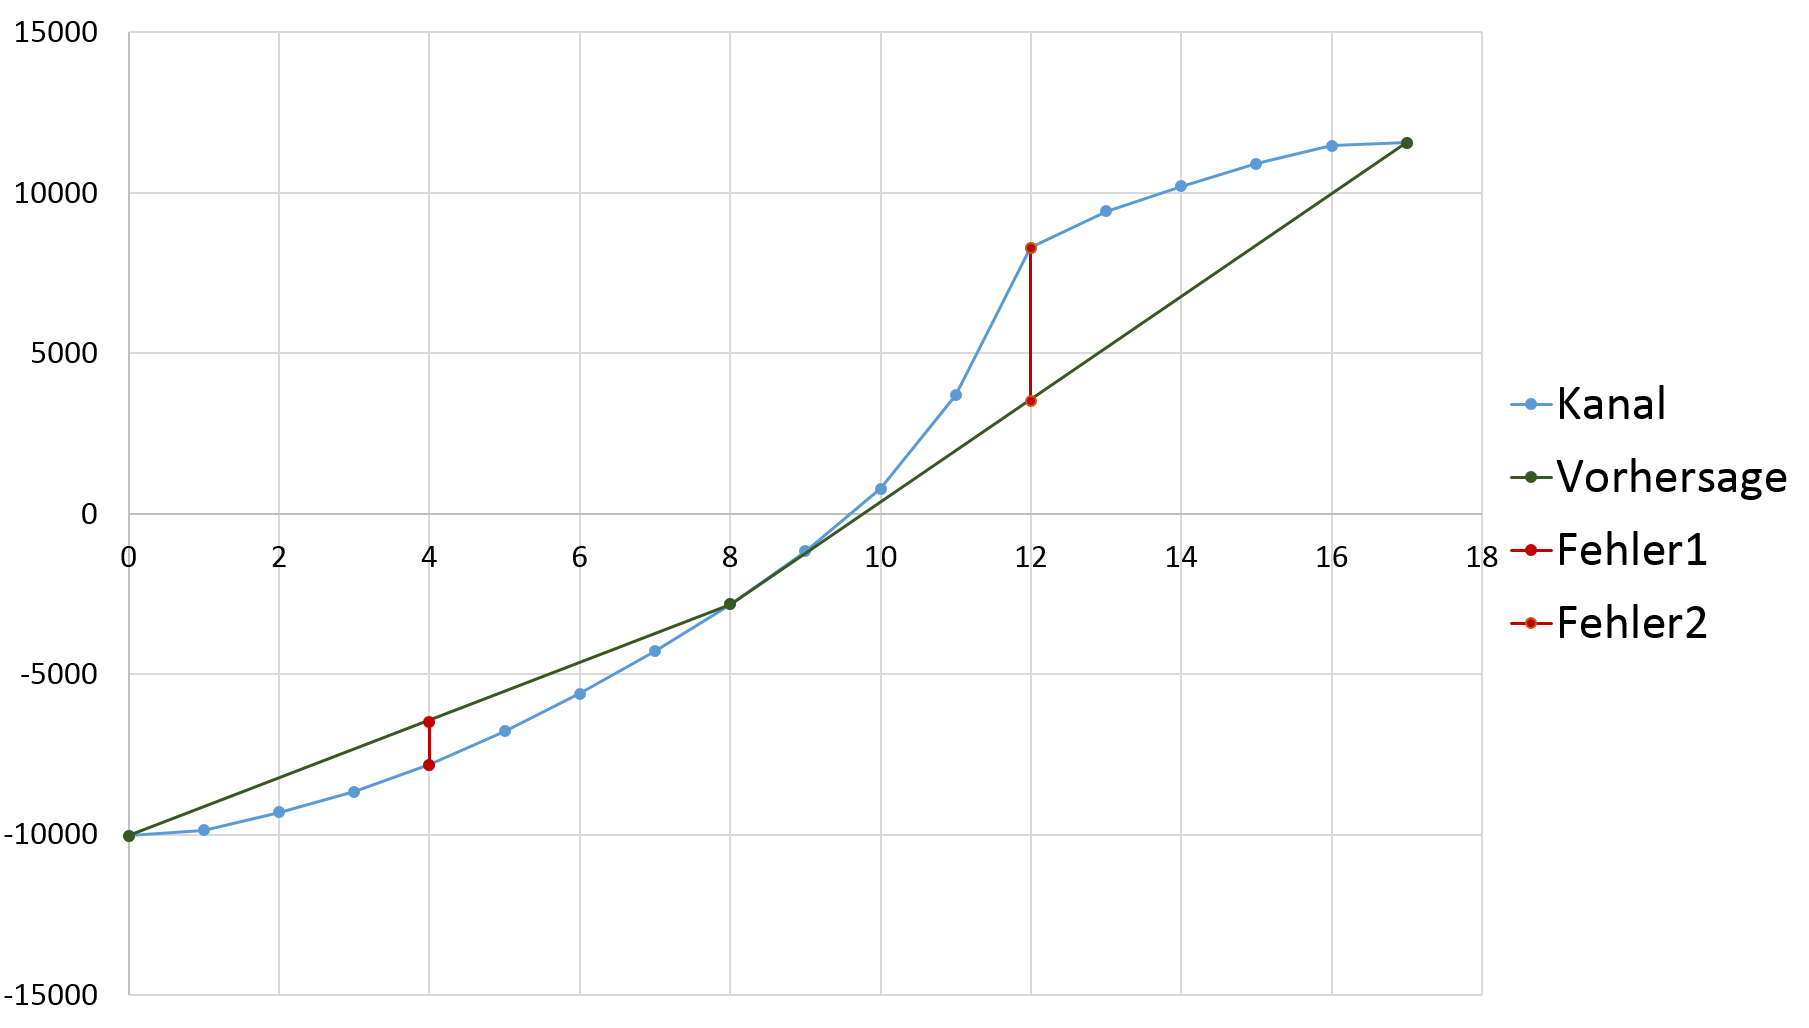
\includegraphics[width=1\textwidth,height=6cm,keepaspectratio]{./pictures/konzept/solution2/algorithm_step2.png}
	\caption{Zweiter Schritt der Wavelet Prediktiven Kodierung. Die Vorhersage beinhaltet nun zwei Strecken.}
	\label{konzept:loesung2:algorithm:step2}
\end{figure} 
wiederholung, bis alles abgelegt ist. Residuals werden immer kleiner

\subsubsection{Quantisierung}
Eine weitere Quantisierung. darf nicht zu viel passieren, sonst geht alles hops. es wurde deshalb noch eine sehr schwache quantisierung eingeführt.

\subsubsection{Entropie Kodierung}
adaptive Kodierung aus DCT. die Längenkodierung wird nicht verwendet, da sie nicht viel auf 0 quantisieren wird. 
\newpage
\section{Qualitätsmessung der Kompression}
Um die Datenmenge der Feldlinien zu verringern werden verlustbehaftete Kompressionsverfahren angewendet. Trotz des Dateverlustes sollen die dekomprimierten Linien möglichst ihren Originalen ähneln. Kleine Abweichungen werden in der Sonnenforschung toleriert. Es ist wichtig, dass die Form der Kurve erhalten bleibt. Grosse, seltene Abweichungen sollten vermieden werden, da sie das Aussehen der Feldlinie verändern können.\\
[\baselineskip]
Zusammen mit Sonnenforschern wurden zwei Fehlermasse bestimmt: Der absolute maximale Fehler und die Standardabweichung von der komprimierten Linie zum Original. Die Standardabweichung ist für diesen Fall geeignet: Grosse, seltene Abweichungen werden stärker gewichtet, als kleine dafür häufige Abweichungen.\\
Der absolute maximale Fehler wird noch als Absicherung gemessen. In den meisten Fällen wird die Kompression mit der tieferen Standardabweichung auch den kleineren maximalen Fehler haben. Da aber die Messung über ein paar hunderttausend Punkte durchgeführt wird, ist das Gegenteil denkbar.\\
Subsample
[\baselineskip]
Eine Grenze für die Genauigkeit ist nicht festzulegen. Auch wenn eine Grenze gefunden wird, kann diese sich in der Zeit verändern. Im Fall der Feldlinien ist die Internetverbindung der Flaschenhals. Es kann sein, dass in Zukunft mehr Präzision bei mehr Platzbedarf verlangt wird. Deshalb werden die Verfahren, wenn möglich, mit unterschiedlichen Qualitätsstufen getestet und verglichen.

\subsection{Auswahl und Erhebung der Testdaten}\label{testsetup:auswahl_erhebung}
Die Testdaten sollen zu einem alle Randfälle abdecken, als auch durchschnittliche Fälle enthalten. Aus diesem Grund wurden insgesamt zehn Datensätze ausgewählt: Vier Datensätze mit hoher Sonnenaktivität, zwei mit wenig und vier zufällig. Für die vier Datensätzen mit hoher Aktivität wurde in den Jahren 2014 und 2013 nach den grössten Solare Flares gesucht. Für die Datensätze mit wenig Aktivität wurde das Gegenteil gemacht, nach Zeiträumen mit möglichst kleinen Solar Flares gesucht.\\
Die feldlinien werden aber nur alle sechs Stunden berechnet und Solar Flares sind sehr spontane Ereignisse. Auch eine grosse Flare kann während den sechs Stunden angefangen und wieder aufgehört haben. Für die grossen Solar Flares wurde deshalb beachtet, dass die Datensätze vor dem Ereignis verwendet wurden. Grosse Solar Flares entladen das Feld, vor dem Ereignis ist das Magnetfeld komplexer.\\
[\baselineskip]
Wie im Abschnitt \ref{konzept:ist-komprimierung} beschrieben, führt der IDL-Code schon eine Quantisierung und ein Subsampling durch. Für die Testdaten wurde das Subsampling und die Quantisierung entfernt. Für jede Dimension eines Punktes wird anstatt 16 Bit 32 Bit Genauigkeit verwendet. Die rohe Datenmenge ist dementsprechend Angewachsen auf etwa 10 MiByte pro Aufnahme.

\subsection{Aublauf des Tests und Messung des Fehlers}\label{testsetup:ablauf}
Float daten werden geladen. Daten kopiert und Kompression/Dekompression durchgeführt für alle Testdaten. Die kopierten Daten wissen aber noch, welches ihr Originalpunkt ist.
Zwei Mengen, Originalpunkte $O$, dekomprimierte Punkte $D$. Es gibt immer gleich viele oder mehr Originalpunkte wie dekomprimierte Punkte. Die Fehlerberechnung muss der allgemeine Fall und die Randbehandlung unterschieden werden.

\subsubsection{Allgemeiner Fall}
\begin{figure}[!htbp]
	\center
	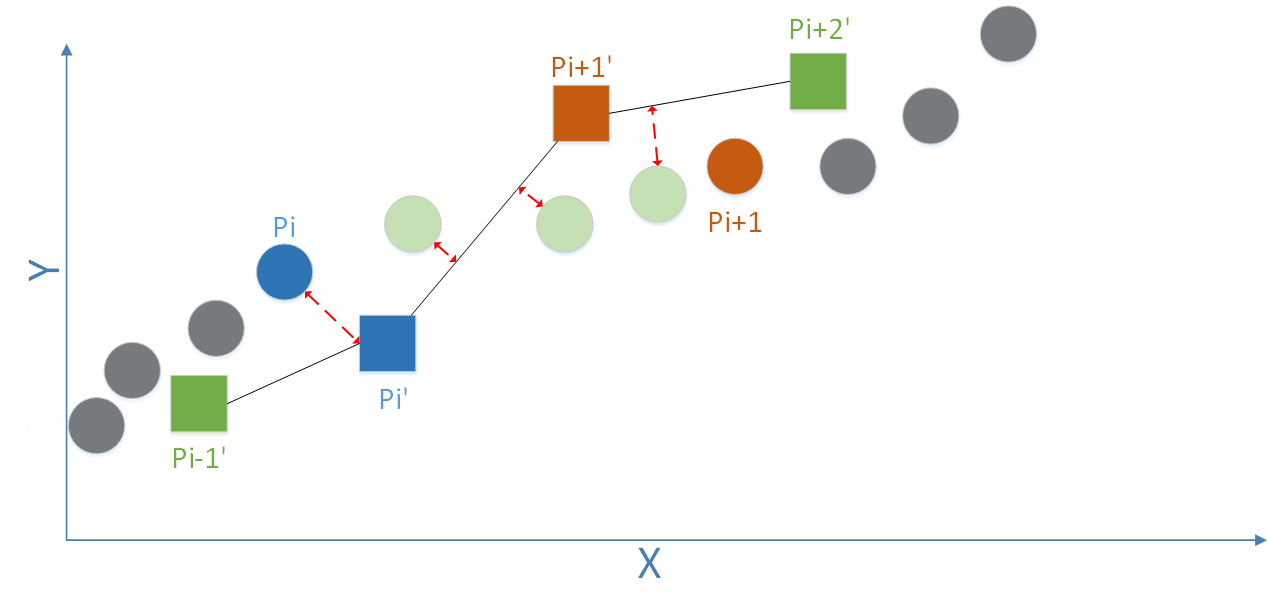
\includegraphics[width=0.8\textwidth,height=6cm,keepaspectratio]{./pictures/testsetup/errorcalc.png}
	\caption{Darstellung der Fehlerberechnung. Die Punkte sind die Originaldaten, die Quadrate sind die Punkte nach der Kompression.}
	\label{testsetup:ablauf:fehlerberechnung:diagramm}
\end{figure} 
Die Berechnung ist Dargestellt im Diagramm \ref{testsetup:ablauf:fehlerberechnung:diagramm}. Für jeden Punkt $p1'$ aus $D$, nehme $p1'$ und den folgenden Punkt und $p2'$. Ziehe eine Strecke $s$ durch $p1'$ und $p2'$. Suche von $p1'$ den Originalpunkt $p1$ aus $O$ und rechne den Abstand aus zur Strecke $s$. Führe das für alle folgenden Originalpunkte durch, bis $p2$ erreicht wurde. Der Abstand $s$ zu $p2$ wird nicht mehr berechnet.\\
[\baselineskip]
\textbf{Abstandsberechnung eines Punktes zu einer Strecke}\\
Gegeben: Stecke $s$ mit Eckpunkten $A$ und $B$ und Punkt $P$.\\
Gesucht: Kürzeste Distanz zwischen $s$ und $P$\\
[\baselineskip]
Zuerst wird überprüft, ob eine Senkrechte durch $P$ überhaupt auf der Strecke $s$ zu liegen kommt. Das ist der Fall, wenn die Strecke $AP$ auf die Strecke $s$ projizierbar ist:
\begin{center}
$ t = \frac{\vec{AB}*\vec{AP}}{\lvert \vec{AB}\rvert ^2}$\\
  $0 \leq t \leq 1$
\end{center}
Wenn das nicht möglich ist, wird der kürzere Distanz von $P$ zu einem der Eckpunkte genommen. Falls aber eine Senkrechte auf $s$ zu liegen kommt, muss jetzt die Länge der Senkrechte berechnet werden. Aus der vorhgehenden Berechnung könnte man den Fusspunkt auf $s$ berechnen und dadurch die Distanz, oder man kann die Distanz direkt über das Kreuzprodukt berechnen.
\begin{center}
  $distance = \frac{\lvert \vec{BA}\times \vec{BP}\rvert}{\lvert \vec{BP} \rvert}$
\end{center}

\subsubsection{Randbehandlung}
\begin{figure}[!htbp]
	\center
	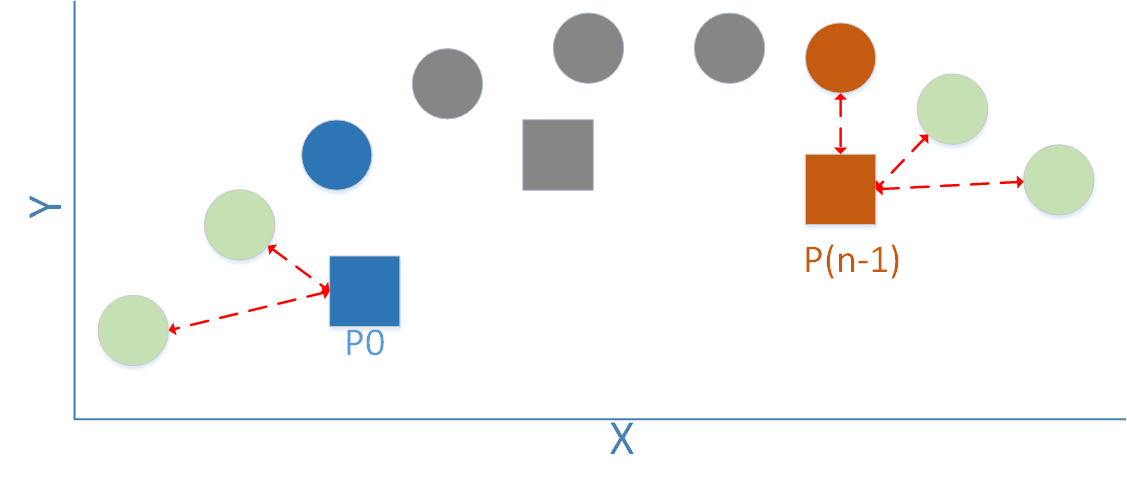
\includegraphics[width=0.8\textwidth,height=6cm,keepaspectratio]{./pictures/testsetup/randbehandlung.png}
	\caption{Darstellung der Fehlerberechnung. Die Punkte sind die Originaldaten, die Quadrate sind die Punkte nach der Kompression.}
	\label{testsetup:ablauf:randbehandlung:diagramm}
\end{figure}
Es ist möglich, dass die originalen Endpunkte durch eine Quantisierung verworfen wurden. Das bedeutet, wenn man den Fehler für den allgemeinen Fall berechnet, am Anfang und am Ende Originalpunkte existieren, für die nie eine Distanz berechnet wurde. Die Abbildung \ref{testsetup:ablauf:randbehandlung:diagramm} zeigt das Problem. Deshalb müssen die Abstände der Ränder von der Komprimierten- zur Original-Linie noch berechnet werden. Der Abstand vom ersten komprimierten Punkt (in der Abbildung P0) zu seinem Original wird schon im allgemeinen Fall berechnet.

\subsubsection{Berechnung der Standardabweichung}
\begin{center}
$\sigma(X) = \sqrt(variance(X))$\\
$variance(X) = \sum{(x_i - E(x_i))^2}$
\end{center}
Die Standardabweichung $\sigma$ einer Beobachtungsreihe $X$ $(x_1,x_2,x_3,\ldots, x_n-1)$ ergibt sich aus der Wurzel der Varianz von $X$. Die Varianz von $X$ kann errechnet werden, wenn man den Distanz jeder Beobachtung $x_i$ mit dem Erwartungswert $E(x_i)$ berechnet und quadriert. Die Beobachtung ist im diesen Fall ein Punkt der dekomprimierten Linie, während der Erwartungswert der Originalpunkt ist. Die Distanz wird mit dem besprochnen Verfahren \ref{testsetup:ablauf} berechnet. Die Summe der quadratischen Abstände ergibt die Varianz. Die Varianz wird über alle Testdaten berechnet, somit erhält man für einen Test genau eine Standardabweichung.
\newpage
\section{Implementation der Dekompression}
Der JHelioviewer lädt eine Folge von komprimierten Simulationen über eine Internetverbindung und muss diese vor der Visualisierung dekomprimieren. Das Herunterladen und die Dekomprimierung sind zeitaufwändige Operationen und kann zu Wartezeiten beim Benutzer führen. Um die Operationen zu beschleunigen werden im Ist-Zustand die Simulationen im Voraus asynchron heruntergeladen. Somit sind die Daten bereits im Arbeitsspeicher, bevor die Daten dekomprimiert und visualisert werden.\\
Die Dekompression wird direkt vor der Visualisierung durchgeführt. Bei einer Animation der Feldliniendaten führt das zu einer bemerkbaren Verzögerung bei jedem Wechsel. Um die Qualität der Animation zu verbessern und die Wartezeit weiter zu verkürzen wurden folgende Massnahmen umgesetzt:
\begin{enumerate}
	\item Asynchrone Dekompression.
	\item Vorladen der Dekomprimierten Feldlinien.
	\item Caching von Komprimierten und Dekomprimierten Feldlinien.
\end{enumerate}

\subsection{Software Architektur}
\begin{figure}[!htbp]
	\center
	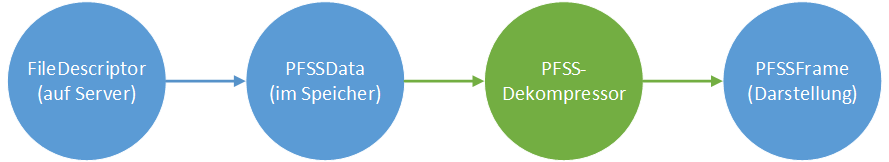
\includegraphics[width=0.6\textwidth,height=6cm,keepaspectratio]{./pictures/implementation/dataflow.png}
	\caption{Zustandsdiagramm der Feldliniendaten}
	\label{implementation:architektur:datenfluss}
\end{figure}
Die Daten der Feldlinien durchlaufen im JHelioviewer vier Zustände, welche durch vier Klassen abgebildet wurden. Die Klassen sowie die Zustandswechsel sind im Diagramm der Abbildung \ref{implementation:architektur:datenfluss} dargestellt. Die Klasse ''FileDescriptor´´ repräsentiert eine Simulation von Feldlinien auf dem Server. In diesem Zustand sind die Daten bereit für das Herunterladen. Die folgende Klasse ''PFSSData´´ symbolisiert Feldlinien, welche in den lokalen Arbeitsspeicher geladen wurden. In diesem Zustand sind die Daten noch komprimiert und nicht bereit für eine Visualisierung. Die Klasse ''PFSSDekompressor´´ ist ein Zwischenzustand und stellt den Wechsel von komprimierten zu unkomprimierten Daten dar. Da der Zustandswechsel aufwändig ist, wird es durch eine eigene Klasse abgebildet. Die letzte Klasse ''PFSSFrame´´ repräsentiert die dekomprimierten Feldlinien. In diesem Zustand sind die Daten bereit für die Darstellung. Die Darstellung wird ebenfalls von der ''PFSSFrame´´ Klasse übernommen.

\subsubsection{Vorladen und Caching von Komprimierten und Dekomprimierten Feldlinien}
Um die Animation der Feldlinien möglichst Unterbrechungsfrei zu gestalten, werden die komprimierten und dekomprimierten Feldliniendaten vorgeladen und gecached. Mit dem Vorladen wird erreicht, dass der Wechsel von der Visualisierung einer Simulation zur anderen möglichst ohne Unterbrechung durchgeführt werden kann. Das Caching hilft, wenn der Benutzer einen anderen Zeitpunkt der Animation nochmals darstellen möchte. Aus dem Zustandsdiagramm der Abbildung \ref{implementation:architektur:datenfluss} kann entnommen werden, dass die Komprimierten Feldlinien von den ''PFSSData'' Objekten und die dekomprimierten Daten von den ''PFSSFrame'' Objekten repräsentiert werden. Die Implementation ist im Diagramm der Abbildung \ref{implementation:architektur:caching} dargestellt.
\begin{figure}[!htbp]
	\center
	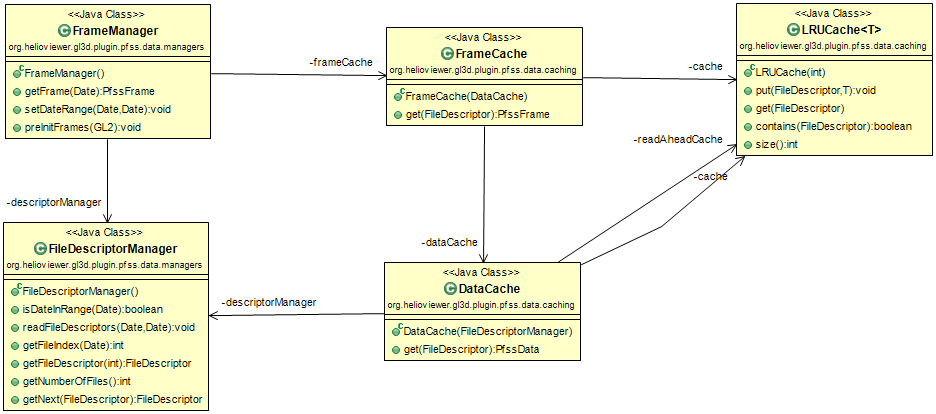
\includegraphics[width=1\textwidth,height=8cm,keepaspectratio]{./pictures/implementation/architectureCache.png}
	\caption{Diagramm der Implementation vom Vorladen und Caching}
	\label{implementation:architektur:caching}
\end{figure}
Die Klasse FrameManager ist zuständig für das Vorladen der dekomprimierten Daten, der PFSSFrame Objekte. Das Caching wird in der FrameCache Klasse umgesetzt. Die Klasse DataCache ist für das Vorladen und Caching der komprimierten Daten zuständig. Die FileDescriptor Objekte repräsentieren eine Feldliniensimulation auf dem Server, der FileDescriptorManager ist zuständig für das Auffinden der Simulationen.\\
Die Klasse FrameManager repräsentiert die Facade der Vorladens- und Caching- Implementation. Sie abstrahiert das Zusammenspiel der verschiedenen Caches und den verschiedenen Zustände der Feldliniendaten und bietet eine vereinfachte Schnittstelle an.\\
Die Vorladen und Caching Implementation der PfssFrame Objekte wurde in zwei Klassen aufgeteilt: Die PfssFrame Objekte müssen vor der Visualisierung Resourcen der Grafikkarte allozieren. Nachdem ein Objekt visualisiert wurde, müssen die Resourcen freigegeben werden. Der FrameManager ist zuständig die Allozierung anzustossen und die Freigabe sicherzustellen.\\
Die PFSSData Objekte können vom Garbage-Collector verwaltet werden. Das Vorladen kann mit einer weiteren Instanz des LRU-Caches umgesetzt werden und wurde direkt in der DataCache Klasse implementiert.

In dieser Arbeit wurde ein Least-Recently-Used (LRU) Cache Algorithmus verwendet. Der LRU-Cache löscht das am längsten nicht verwendete Objekt, wenn der Cache gefüllt ist. Da der JHelioviewer im allgemeinen Fall sequenzell Objekte verlangt, kann der LRU Cache mit einer First-in-First-Out Queue implementiert werden. Das Objet, welches am längsten nicht  verwendet wurde, ist das Letzte in der Queue. Ein LRU-Cache funktioniert in diesem Anwendungsfall optimal, wenn die Anzahl Objekte grösser ist, als der Cache. In einem Spezialfall ist der LRU-Algorithmus nicht optimal. Wenn der JHelioviewer zur letzten Simulation der Feldlinien angekommen ist, wird an Wrap-around durchgeführt und wieder die erste Simulation verlangt. Wenn der Cache $n-1$ von $n$ Simulation abspeichern kann, so löscht der LRU-Algorithmus immer die Simulation, welches als übernächstes abgefragt wird. Das führt dazu, dass gleich viele Cache-Misses geschehen, als wenn der Cache wesentlich kleiner währe.

\subsubsection{Asynchrone Aufrufe mittels Executor Services}
Im Diagramm der Abbildung \ref{implementation:architektur:caching} zu sehen ist, wird das Erstellen von PFSSData und PFSSFrame Objekten jeweils von zwei Klassen übernommen werden, den Creators. Sie sind zuständig für das asynchrone Herunterladen und Dekomprimieren der Feldliniendaten. Die asynchrone Ausführung ist mit dem Java Executor Service umgesetzt. Der Executor Service verwaltet und begrenzt die Anzahl an Threads welche die Aufrufe bearbeiten, sodass auch bei hoher Auslastung ein möglichst hoher Durchsatz erreicht wird. Im Ist-Zustand wurden alle asynchrone Aufrufe jeweils in einem eigenen Thread ausgeführt. Bei hoher Auslastung steigt der Verwaltungsaufwand der Threads und bremst das System.\\
\newpage
\section{Resultate}\label{resultate}
Es gibt x Lösungenansätze mit x varianten.  hier sind die Kompressionsraten der jeweils besten Varianten der Ansätze.\\
Bis auf den Lösungsansatz unter \ref{resultate:loesung0} Unterschiedliche Qualitätsstufen

\subsection{Lösungsansatz: Angle-Subsampling} \label{resultate:loesung0}
Bild
Der Ist-Zustand wird das Angle-Subsampling\footnote{siehe Abschnitt \ref{konzept:loesung0:subsampling}} im JHelioviewer durchgeführt. Diese Variante führt das Subsampling vor der Dateiübertragung durch. Die resultierende FITS-Datei wird mittels Rar kodiert\footnote{siehe Abschnitt\ref{konzept:loesung0:kodierung}};
\begin{figure}[!htbp]
	\center
	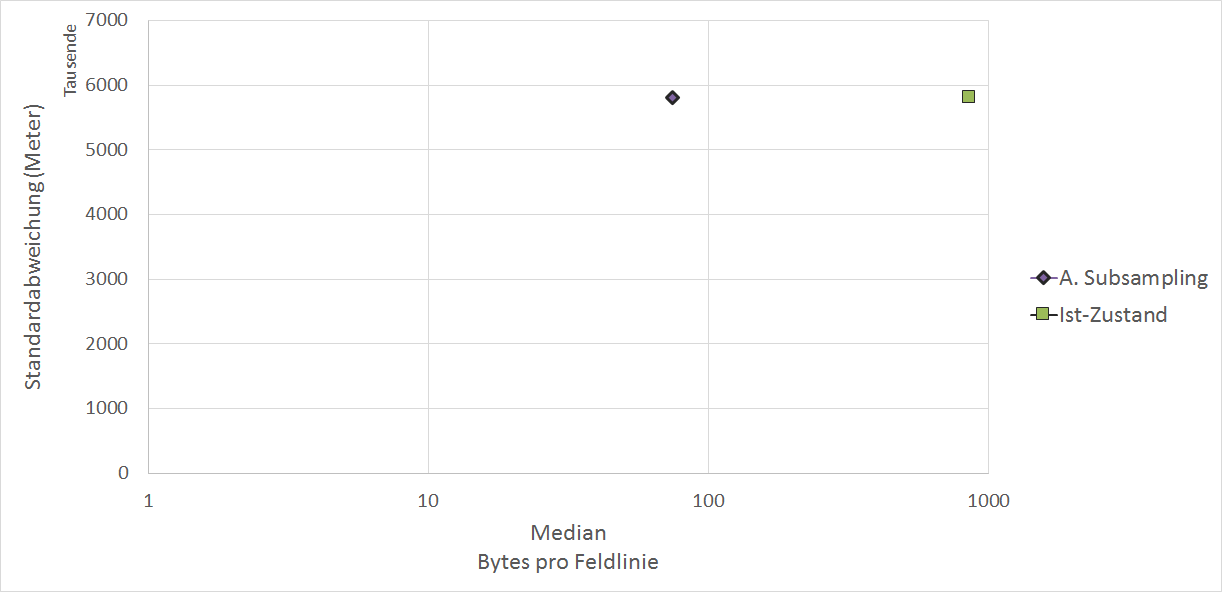
\includegraphics[width=0.8\textwidth,height=6cm,keepaspectratio]{./pictures/resultate/loesung0/loesung0_0.png}
	\caption{Vergleich der Lösung 0 zum Ist-Zustand.}
	\label{resultate:loesung0:loesung0_0}
\end{figure}
%Grösse der DAtei
Wie im Diagramm \ref{resultate:loesung0:loesung0_0} erkennbar ist, verbraucht die Lösung 0 deutlich weniger Speicher. Das Angle-Subsampling reduziert deutlich die Anzahl Punkte, während die Rar eine bessere Kompression erbringt. Die Komplexität der Kompression und Dekompression bleibt in der Grössenordnung $O(n)$ ($n$ ist die Anzahl Punkte). Da bei der Dekompression $n$ etwa vier Mal weniger Punkte bearbeiten muss, ist die Dekompression sogar schneller als die Ist-Lösung.\\
\begin{figure}[!htbp]
	\center
	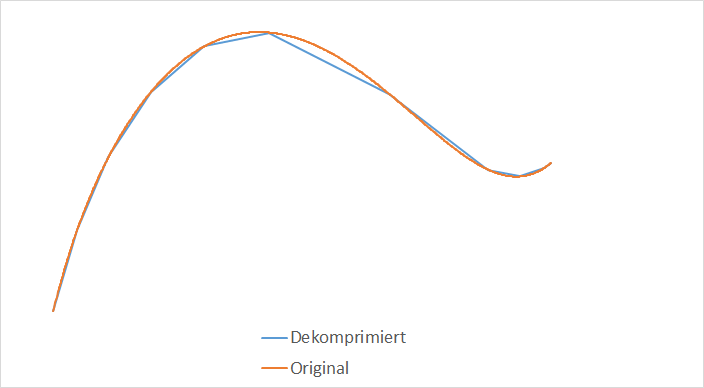
\includegraphics[width=0.8\textwidth,height=6cm,keepaspectratio]{./pictures/resultate/loesung0/loesung0_artefakte.png}
	\caption{Artefakte der Lösung 0}
	\label{resultate:loesung0:artefakte}
\end{figure}
Die Abbildung \ref{resultate:loesung0:artefakte} zeigt die Artefakte, die bei der Komprimierung der Lösung 0 entstehen. Es ist anzumerken, dass der Ist-Zustand die selben Artefakte aufweist.

\subsection{Lösungansatz: Diskrete Kosinus Transformation}
Lösungsvarianten
d
In den folgenden Abschnitten werden die Resultate verschiedener Varianten vorgestellt. Alle Varianten bestehen grob aus fünf Teilschritten: Einem Subsampling\footnote{siehe Abschnitt \ref{konzept:loesung1:subsampling}}, einer Folge von verschiedenen Transformationen, bei der eine die Diskrete Kosinus Transformation ist, Abspeicherung ins Fits Format\footnote{siehe Abschnitt \ref{konzept:loesung0:fits}} undeiner Quantisierung und einer Entropie Kodierung mit Rar\footnote{siehe Abschnitt \ref{konzept:loesung0:kodierung}}.\\
[\baselineskip]
In den Tests wurde eine lineare Quantisierung verwendet. Jeder DCT Koeffizient wird durch einen Faktor geteilt, der sich stetig ehöht. Zum Beispiel wird der erste Koeffizient durch zwei geteilt, der zweite durch Vier, der Dritte durch Sechse etc.  Die Kompressionsrate kann durch einen höheren oder tieferen Faktor gesteuert werden. Diese Quantifizierung ist nicht das Optimum. Eine bessere Quantifizierung wird für die beste Lösung ausgearbeitet.

\subsubsection{Variante: DCT}\label{resultate:dct}
Bild
verwendet als Transformation nur DCT. Eizige Veränderung, jeder Kanal wird mit 32 Bit Integer anstatt mit 16 Bit abgespeichert. DCT-Koeffizienten sind sonst zu gross.
\begin{figure}[!htbp]
	\center
	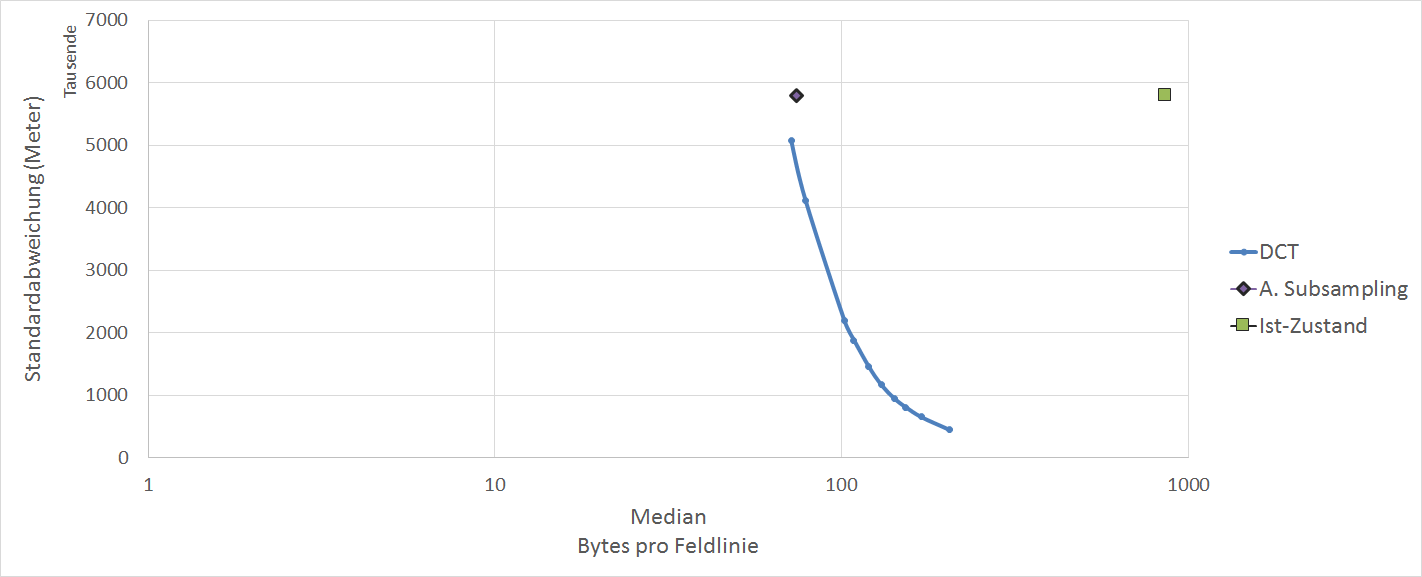
\includegraphics[width=0.8\textwidth,height=6cm,keepaspectratio]{./pictures/resultate/loesung1/loesung1-0/loesung1_0.png}
	\caption{Vergleich der DCT Kompression mit der Lösung0}
	\label{resultate:loesung1:dct:resultate}
\end{figure}
Die Abbildung \ref{resultate:loesung1:dct:resultate} zeigt den Vergleich der DCT Kompression mit der Lösung 0. Es ist deutlich zu erkennen, dass die Standardabweichung schnell steigt bei leicht sinkender Grösse. Der Maximale Fehler ist ist mehr als vier Mal grösser, als die der Lösungsvariante \ref{resultate:loesung0} steigt ebenfalls schnell und erreicht beim letzten Test eine höhe von $140'686'000$ Meter. Zum Vergleich: Der maximale Fehler der Lösung 0 ist mehr als vier Mal kleiner und liegt bei $30'014'000$ Meter.\\
\begin{figure}[!htbp]
	\center
	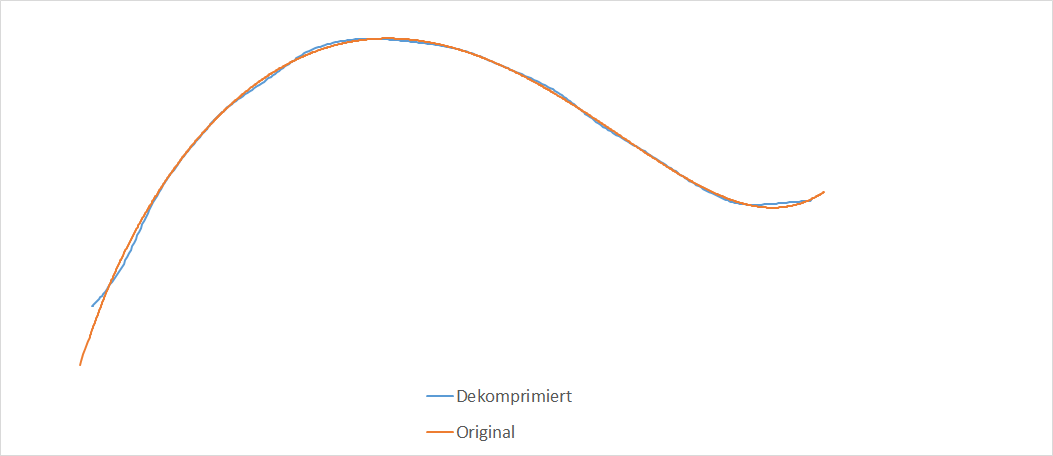
\includegraphics[width=0.8\textwidth,height=6cm,keepaspectratio]{./pictures/resultate/loesung1/loesung1-0/loesung1_0_artefakte.png}
	\caption{Artefakte der DCT Dekompression anhand Beispieldaten}
	\label{resultate:loesung1:dct:artefakte}
\end{figure}
Die Darstellung der Artefakte \ref{resultate:loesung1:dct:artefakte} zeigen das Problem: in den meisten Fällen kann die DCT die Feldlinie gut approximieren. Bei dieser Feldlinie wird der Anfang der Kurve nicht richtig dargestellt. Das ist ein typisches Problem der DCT. In diesem Fall wird für die Transformation angenommen, dass sich das Signal am Anfang und am Ende in umgekehrter Reihenfolge wiederholt \cite{wiki:dct}. Das führt am Anfang der Kurve zu einer grossen Spitze, welche sich nur durch sehr hochfrequente Schwingungen darstellen lässt.  Wenn diese Anteile durch die Quantisierung verschwinden, entstehen solche Artefatkte.\\
Eine Möglichkeit ist die Feldlinie um Punkte zu erweitern. Wenn die Feldlinie am Anfang und am Ende abflacht, sollte die resultierende Transformation weniger hochfrequente Schwingungen enthalten. Durch eine andere Darstellung könnten diese Probleme ebenfalls gelöst werden.

\subsubsection{Variante: Ableitung+DCT}\label{resultate:dct:ableitung_dct}
Bild
Bevor die Feldlinie Kosinus-Transformiert und Quantisiert wird, soll sie abgeleitet werden. Dämpfung der koeffizienten, die diskretisierten Koeffizienten sollten weniger speicherplatz verbrauchen. Mit der Ableitung soll das Randproblem dargestellt in \ref{resultate:loesung1:dct:artefakte} gelöst werden. Die Steigungen sind kleinere Zahlen, was an den Rändern keine grosse Spitze verursachen sollte. Der Nachteil ist, dass Ungenauigkeiten sich durch die Kurve durchziehen und summieren.\\
Damit die Ableitung umkehrbar ist, wird neu jeder Startpunkt der Feldlinie mit in die Fits Datei abgelegt. Die DCT-Koeffizienten werden mit 16 Bit Genauigkeit abgelegt.\\

\begin{figure}[!htbp]
	\center
	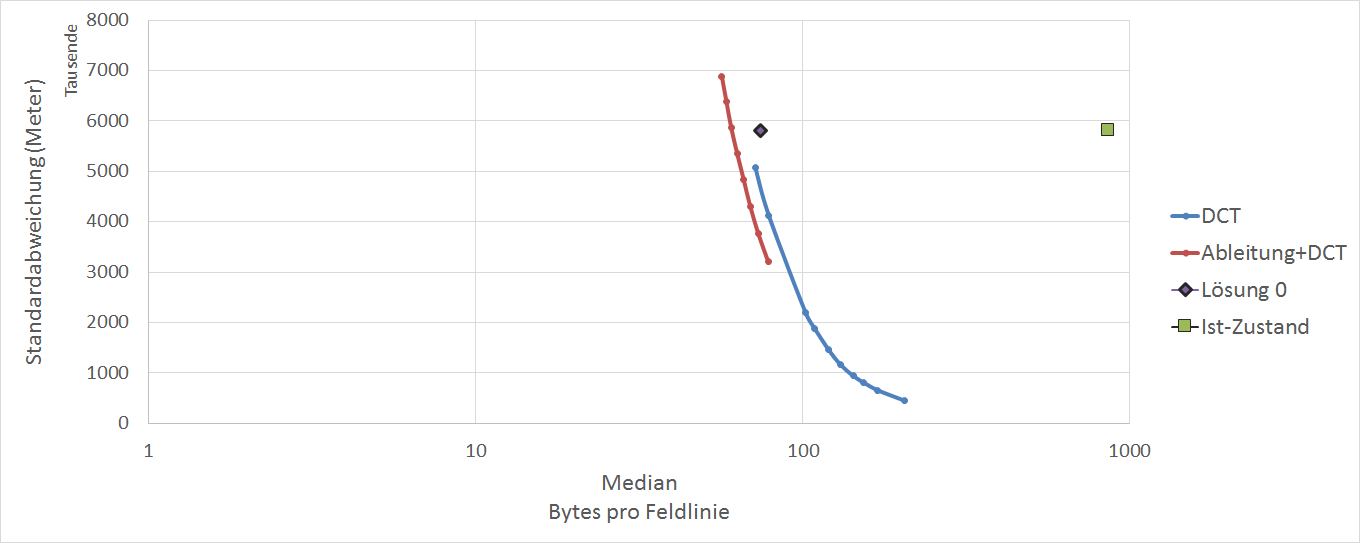
\includegraphics[width=0.8\textwidth,height=6cm,keepaspectratio]{./pictures/resultate/loesung1/loesung1-1/loesung1_1.png}
	\caption{Vergleich der DCT Kompression der Ableitung mit der DCT Kompression}
	\label{resultate:loesung1:dct:artefakte}
\end{figure}
Die abgeleiteten Feldlinien können sehr gut quantisiert werden. Im Vergleich zur Lösung 0 braucht diese Variante etwa $15$ Byte weniger um eine Feldlinie darzustellen. Durchschnittlich ist jetzt eine PFSS Simulation auf $72$ KiByte komprimiert. Die Ränder können dargestellt werden, eine Darstellung der Artefakte ist auf der Abbildung \ref{resultate:loesung1:dct:byte:artefakte} zu finden.\\
Die Feldlinien liegen meist auf einer Ebene im dreidimensionalen Raum. Wenn die X,Y und Z Kanäle Kosinus-Transformiert werden, ist die Information etwa gleichmässig auf den Kanälen verteilt. Eine Linie könnte sich durch weniger Kosinus-Funktionen approximieren lassen, wenn die Linie zuerst in ein lokales Koordinatensystem transformiert wird. Die Koordinatenachsen können für jede Linie so gelegt werden, dass der X und Y Kanal den grossteil der Informationen beinhalten. Es wird vermutet, dass für Approximation des X und Y Kanals mit etwa gleich viele Kosinus-Funktionen gebraucht werden, aber für den Z Kanal bedeutend weniger.

\subsubsection{Variante: Ableitung+PCA+DCT}
Bild
Die Principal Component Analysis (PCA)\cite{abdi2010principal} ist ein Verfahren aus der Statistik, welches Daten in ein neues koordinatensystem Transformiert. Dabei werden die Achsen so gelegt, dass die Daten entlang der ersten Achse die grösste Varianz aufweisen. Entlang der zweiten Achse, welche orthogonal zur ersten liegt, die zweithöchste Varianz etc. Wenn das Vefahren auf die Feldlinien angewandt wird, werden die Feldlinien in ein lokales System transformiert indem der Z-Kanal 0 ist, wenn die Feldlinie in einer Ebene liegt. Der Nachteil ist, dass für die Rücktransformation pro Feldlinie die Koordinatenachsen und die Koordinatenverschiebung abgespeichert werden.\\
Vor der DCT wird nun eine PCA durchgeführt. Die sechs Faktoren der neuen Koordinatenachsen werdenmit  16 Bit Genauigkeit in die Fits-Datei abgelegt und die drei Verschiebung-Faktoren mit 32 Bit.
\begin{figure}[!htbp]
	\center
	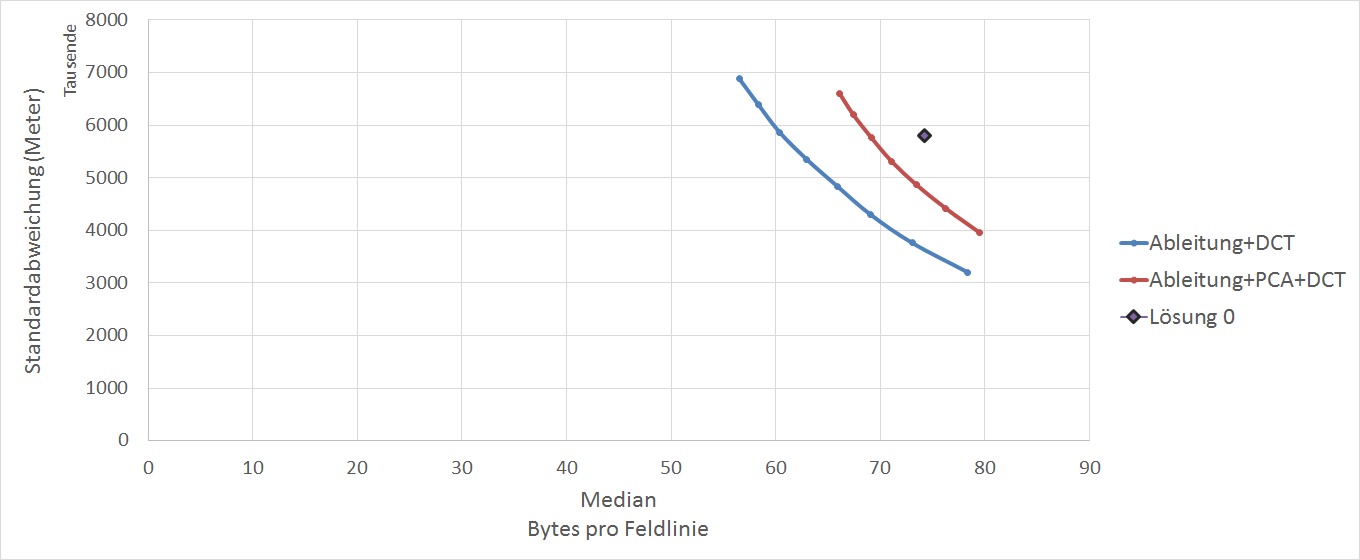
\includegraphics[width=0.8\textwidth,height=6cm,keepaspectratio]{./pictures/resultate/loesung1/loesung1-4/loesung1_4.png}
	\caption{Vergleich der PCA DCT Kompression der Ableitung mit der DCT Kompression der Ableitung}
	\label{resultate:loesung1:dct:pca}
\end{figure}
Der Vergleich \ref{resultate:loesung1:dct:pca} zeigt deutlich, dass sich der Mehraufwand nicht lohnt, obwohl die PCA vielversprechend scheint. Eine Feldlinie lässt sich mit 5 bis maximal 20 Kosinus-Funktionen pro Kanal approximieren. Durch die PCA-Transformation lässt sich das noch minim verkleinern, aber die zusätzlichen Informationen wie die Werte für neuen Koordinatenachsen und für die Verschiebung verbrauchen mehr speicher, als durch die Transformation gewonnen werden kann.\\
Die PCA-Variante könnte noch verkleinert werden. Die Verschiebung kann Quantisiert werden, oder man kann weniger Genauigkeit für die Koordinatenachsen verwenden. Die PCA-Variante ist aber nicht genauer wie die Ableitung+DCT Variante. Wie auch in \ref{resultate:loesung1:dct:pca} ersichtlich, ist die PCA-Variante bei vergleichbarer Kompressionsgrad ungenauer. Unter dem Strich hat die PCA keine Verbesserung erbracht.\\
[\baselineskip]
Es gibt weitere Transformationen, welche die Feldlinien so darstellen, dass weniger Kosinus-Funktionen für die selbe Approximation gebraucht werden. Die Transformationen brauchen aber für die Rückwärds-Operation meist zusätzliche Informationen. Zusätzlich bringen führen weitere Transformationen Ungenauigkeiten wie Rundungsfehler mit sich. Bei 5 bis 20 Kosinus-Funktionen pro Kanal ist es schwierig eine Transformation zu entwickeln, welche mindestens so genau ist und dabei weniger Speicherplatz verbraucht. Die ganze Kodierung wird momentan Rar überlassen. Dort gibt es noch Optimierungspotential.

\subsubsection{Variante: Ableitung+DCT+Byte Kodierung} \label{resultate:loesung1:ableitung_dct_kodierung}
Es wird versucht, mit einer Byte Kodierung die DCT-Koeffizienten der Variante \ref{resultate:dct:ableitung_dct} besser zu komprimieren. Die Koeffizenten werden mit zwei Verfahren kodiert: Mit einer simplen Run-Length Kodierung und einer adaptiven Byte Kodierung. Die adaptive Byte Kodierung versucht jeden koeffizienten mit einem Byte darzustellen. Wenn die Genauigkeit nicht ausreicht, wird ein weiteres Byte hinzugenommen. Die Kodierung ist im Abschnitt \ref{konzept:loesung1:kodierung} beschrieben.
\begin{figure}[!htbp]
	\center
	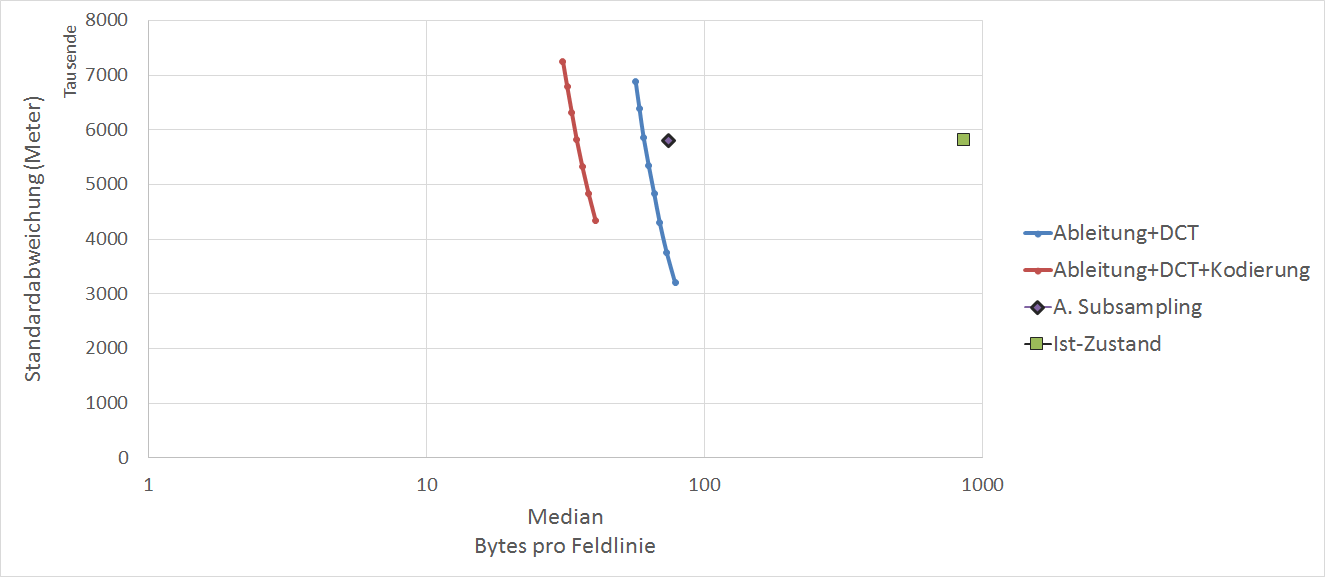
\includegraphics[width=0.8\textwidth,height=6cm,keepaspectratio]{./pictures/resultate/loesung1/loesung1-6/loesung1_6.png}
	\caption{Vergleich der Kompression mit und ohne Byte-Kodierung}
	\label{resultate:loesung1:dct:kodierung}
\end{figure}
\ref{resultate:loesung1:dct:kodierung} zeigt eine deutliche Verbesserung der Kompressionsrate, wenn die Koeffizienten mit der unter \ref{konzept:loesung1:kodierung} beschriebenen Verfahren kodiert werden. Bei ähnlicher Genauigkeit wie der Ist-Zustand braucht diese Variante durchschnittlich $35$ Bytes pro Feldlinie. Bei $1200$ Feldlinien eine ergibt das eine Dateigrösse von $42$ KiByte pro Aufnahme. Im Vergleich zum Ist-Zustand sind die Dateien um das 24 Fache kleiner.\\
[\baselineskip]
Bei der Variante \ref{resultate:dct} war das Problem, dass die Ränder schlecht darzustellen waren. Es stellt sich die Frage, was für Artefakte diese Kompression aufweist.
\begin{figure}[!htbp]
	\center
	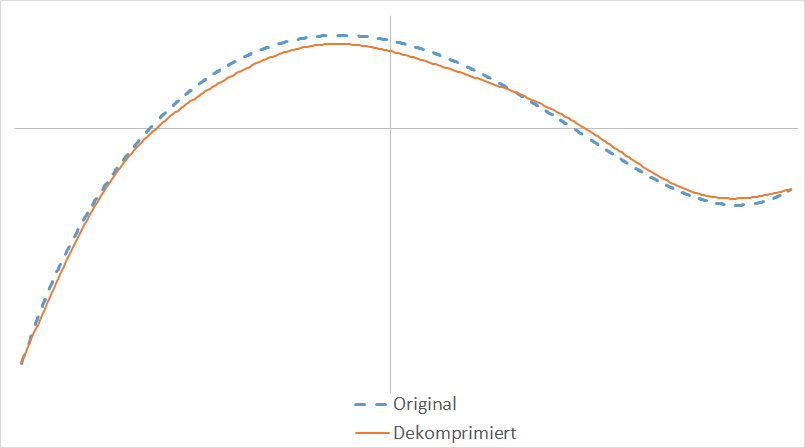
\includegraphics[width=0.8\textwidth,height=6cm,keepaspectratio]{./pictures/resultate/loesung1/loesung1-6/artefakte.png}
	\caption{Artefakte der DCT Kompression der Ableitung}
	\label{resultate:loesung1:dct:byte:artefakte}
\end{figure} 
Die Abweichung ist in der selben Grössenordnung wie die der Lösung 0. In der Abbildung\ref{resultate:loesung1:dct:byte:artefakte} ist deutlich zu sehen, dass die Kurve durch die Quantisierung gedämpft wird. Die Maximum der Kurve ist tiefer, sowie das lokale Minima der letzten Halbwelle höher. Der Vorteil dieser Variante ist, dass die resultierende Feldline sehr glatt verläuft. Ohne die Originalkurve währen die Artefakte nicht zu identifizieren.\\
Wenn man die Artefakte von \ref{resultate:loesung1:dct:byte:artefakte} und \ref{resultate:loesung0:artefakte} vergleicht, fällt auf dass die Variante \ref{resultate:dct} die Feldlinie genauer approximiert. Wenn die Ränder besser dargestellt werden, ist es Denkbar, dass die Variante \ref{resultate:dct} wenigere Kosinus-Funktionen braucht für eine ähnlich genaue Approximation.

\subsubsection{Variante: DCT+Byte Kodierung}
Wieder nur die Diskrete Kosinus Transformation, aber noch mit künstlich erzeugten Punkten\ref{konzept:loesung1:randbehandlung} und der Byte Kodierung\ref{konzept:loesung1:kodierung}.
\begin{figure}[!htbp]
	\center
	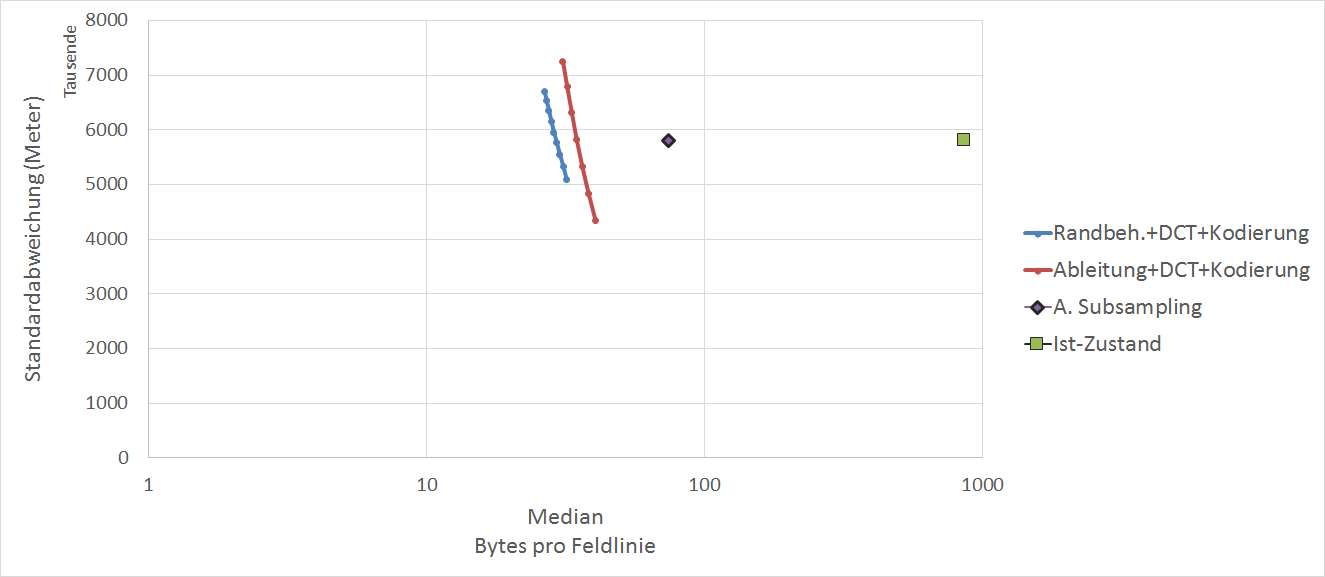
\includegraphics[width=0.8\textwidth,height=6cm,keepaspectratio]{./pictures/resultate/loesung1/loesung1-7/loesung1_7.png}
	\caption{Vergleich der Kompression mit und ohne Byte-Kodierung}
	\label{resultate:loesung1:dct:randbehandlung}
\end{figure}
Noch besser, noch wenige Bytes pro feldlinie
\begin{figure}[!htbp]
	\center
	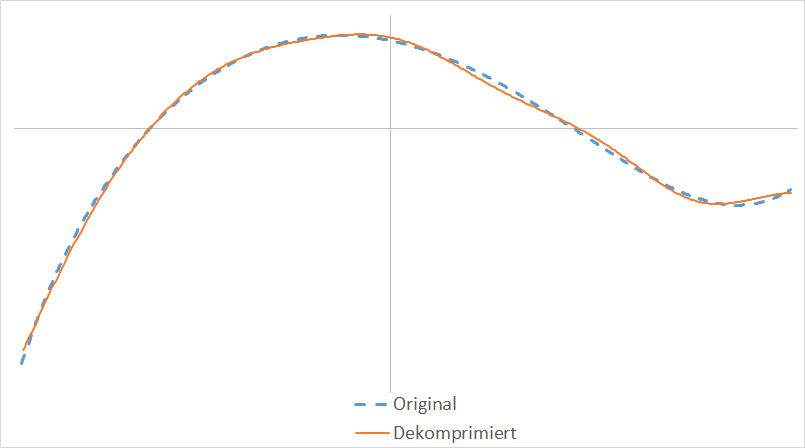
\includegraphics[width=0.8\textwidth,height=6cm,keepaspectratio]{./pictures/resultate/loesung1/loesung1-7/artefakte.png}
	\caption{Artefakte der DCT Kompression der Ableitung}
	\label{resultate:loesung1:dct:randbehandlung:artefakte:}
\end{figure} 
Randbehandlung noch nicht Perfekt.
Artefakte wird man bei der Visualiserung nicht bemerken, da sowieso nicht alle Punkte dargestellt werden können. Artefakte andere Eigenschaft wie \ref{resultate:loesung1:ableitung_dct_kodierung}, sie könnten als solches Enttarnt werden.

Realität sieht aber anders aus, überall kleine schwingungen. Visuell nicht schön anzuschauen. Kompression ist nicht brauchbar.
Bild Umsetzung
In diesem Fall scheint die Genauigkeitsmetrik versagt zu haben. Man kann es noch retten, aber braucht sehr viel mehr Informationen. Bereits bei 59 Bytes per Pixel.
Bild verbesserung
Entscheidung, auf VAriante 6 umzusteigen. Diese Lösung scheint unter dem selben Problem zu leiden, aber weitaus weniger extrem. DAs Bedeutet, dass das Fehlermass schlecht ist und geändert werden soll. Deshalb wurde eine neue Metrik entwickelt, welche unter\ref{testsetup:psnr}


\subsubsection{Variante:Bla}
Für diesen FAll quantisierung angepasst, aber selbst d

\newpage
\section{Diskussion}

\subsection{Lösungsansatz Adaptives Subsampling}
Der Lösungsansatz des adaptiven Subsamplings erreicht eine Kompressionsrate von $11.6$ gegenüber dem Ist-Zustand, indem es nur die Punkte überträgt, welche der JHelioviewers darstellt. Dadurch sind die visualisierten Feldlinie der Ist-Kompression mit diesem Lösungsansatz identisch. In Zukunft ist es aber denkbar, dass im JHelioviewer deutlich mehr Punkte dargestellt werden sollen. In diesem Fall müssen entweder mehr Punkte übertragen werden oder der JHelioviewer mit einer Interpolation erweitert werden.

Der JHelioviewer muss in der Lage sein $1000$ komprimierte Simulationen im Arbeitsspeicher abzulegen. Mit dieser Kompression werden durchschnittlich $85$ Megabyte an Arbeitsspeicher benötigt. Wenn von einer $10$ Megabit Internetverbindung ausgegangen wird, werden für das Herunterladen von $1000$ Simulationen $70$ Sekunden benötigt. Das ist eine deutliche Verbesserung gegenüber zum Ist-Zustand, welcher unter den selben Bedingungen $790$ Sekunden ($13$ Minuten) benötigt. Mit dieser Kompression können etwa $14$ komprimierte Simulationen pro Sekunde übertragen werden. Der Benutzer erhält eine flüssige Animation der Feldlinien, wenn pro Sekunde weniger als $14$ unterschiedliche Simulationen angezeigt werden müssen.

Ein Vorteil dieses Lösungsansatzes ist die Laufzeit Dekompression: Da keine rechenaufwändige Transformationen verwendet werden braucht dieser Lösungsansatz $19$ Millisekunden für eine Dekompression (Siehe Abschnitt \ref{anhang:performance}). Mit einem Thread ist die Testmaschine in der Lage $50$ Simulationen pro Sekunde zu dekomprimieren. Anders als der DCT Lösungsansatz wird für die Dekompression keine Parameter zwischengespeichert. Dieser Lösungsansatz verbraucht für die Dekompression am wenigsten Ressourcen, vorausgesetzt dass keine Interpolation benötigt wird.

\subsection{Lösungsansatz Diskrete Kosinus Transformation}
Die DCT Kompression kann eine Kompressionsrate von $14.1$ erreicht werden. Im Vergleich mit dem Lösungsansatz des adaptiven Subsampling wird eine höhere Kompressionsrate erreicht, obwohl eine höhere Anzahl an Punkte übertragen werden. Die Problematik dieses Ansatzes liegt darin, dass die DCT Kompression Ringing Artefakte hinzufügt (siehe Abschnitt \ref{resultate:loesung1:ringing}). Die Artefakte können bei allen Kompressionsverfahren mit einer Kosinus Transformation auftreten, wie bei JPEG/JFIF Bilder und MP3 Audiodateien. Der JHelioviewer bietet die Möglichkeit, an die Feldlinien heranzuzoomen. Sobald Ringing Artefakte existieren ist der Benutzer in der Lage sie zu finden. Bei der Entwicklung der Kompression wurde nach Möglichkeiten gesucht, die Ringing Artefakte zu dämpfen. Die Daten sind Artefaktfrei bei etwa der Hälfte des Zoombereichs. Mit einer Glättung der Feldlinien konnten die Ringing Artefakte für alle Zoomstufen behoben werden. In der Bildverarbeitung wird nach weiteren Post-Processing Methoden geforscht, welche Ringing Artefakte vermindern. Die Qualität oder die Kompressionsrate könnte durch ein angepasstes Post-Processing weiter verbessert werden. Eine andere Möglichkeit ist die Diskrete Kosinus Transformation durch eine Wavelet Transformation zu ersetzen. Die Wavelets sind im Allgemeinen weniger Anfällig auf Ringing Artefakte und haben das Potential eine ähnliche Kompressionrate zu erreichen ohne Ringing Artefakte einzuführen.

Beim Caching von $1000$ Simulationen benötigt dieser Ansatz $70$ Megabyte Arbeitsspeicher, etwa $15$ Megabyte weniger als der Lösungsansatz des adaptiven Subsamplings. Wenn von der selben $10$ Megabit Internenetverbindung ausgegangen wird, werden $56$ Sekunden benötigt um $1000$ Simulationen herunterzuladen. Pro Sekunde werden $17$ anstatt $14$ Simulationen übertragen. Wenn für die Movies auf einen artefaktfreien Zoom verzichtet wird, ist eine höhere Kompressionsrate möglich.

Die bessere Kompressionsrate kommt auf Kosten der Komplexität der Dekompression. Die Laufzeit der Dekompression hängt im Wesentlichen von der Implementation der inversen DCT ab. Eine naive Implementation braucht für eine Dekompression etwa drei Sekunden. Die grösste Zeit wird in der Berechnung der Kosinus-Werte verbraucht. Bei der Implementation in dieser Arbeit werden die Kosinus-Werte über SoftReferences gecached. Der Cache passt sich somit an den Arbeitsspeicher an. Wie schnell die Dekompression ist, hängt im Wesentlichen vom verfügbaren Arbeitsspeicher ab. Im besten Fall ergibt das eine Laufzeit von $65$ Millisekunden und im schlechtesten Fall $350$, was zu einem Durchsatz zwischen $3$ und $15$ Simulationen pro Sekunde pro Thread führt.

\subsection{Lösungsansatz Prediktive Kodierung}
Das Caching von $1000$ Simulationen verbraucht mit diesem Ansatz $78$ Megabyte an Arbeitsspeicher Die Übertragungszeit von $1000$ Simulationen beträgt  $62$ Sekunden und die Übertragungsrate, liegt bei $16$ Simulationen pro Sekunde. Die Kompressionsrate fällt zwischen zwischen dem DCT und dem adaptiven Subsampling Ansatz. Die Laufzeit der Dekompression fällt mit $1$ Millisekunden pro Simulation ebenfalls zwischen den beiden Ansätzen. Im Durchschnitt kann ein einzelner Thread $32$ Simulationen pro Sekunde dekomprimieren.

Die Artefakte der Dekompression sind meistens für das menschliche Auge unsichtbar. Es können leichte Verschiebungen einzelner Punkte auftreten, welche erst bei maximaler Zoomstufe als Artefakte erkennbar werden. Mit einer Glättung können die letzten Anzeichen von Artefakten versteckt werden. 

Der Lösungsansatz der 
Sind Artefakte genügen klein um die tiefere Kompression zu rechtfertigen?  Wie kann diese Variante verbessert werden?
Vorteil: einfache
\newpage
\section{Fazit}
Die Ist-Kompression benötigt durchschnittlich 1 Megabyte an Daten pro Simulation der Feldlinien. Das Caching von $1000$ Simulationen verbraucht ein Gigabyte an Arbeitsspeicher. Da der Arbeitsspeicher ebenfalls für die Zwischenspeicherung weiterer Daten benötigt wird, ist diese Datenmenge nicht vertretbar. Um das Zwischenspeichern der Simulationen zu ermöglichen, ist eine Kompressionsrate von Faktor $8-10$ notwendig. Die entwickelten Kompressionsverfahren Adaptives Subsampling, DCT Kompression und Prädiktive Kodierung erreichten eine Kompressionsrate von $11.6$, $14.1$ und $13.6$. Das Zwischenspeichern von $1000$ Simulationen benötigt zwischen $70$ und $85$ Megabyte Arbeitsspeicher. Somit ist das Caching mit allen entwickelten Kompressionsverfahren realisierbar.

Ein Forschungsziel ist, unter welchen Bedingungen ein Streaming der Simulationen möglich ist. Es wird angenommen, dass für die Feldlinien $5$ Megabit Bandbreite zur Verfügung stehen. Mit dieser Bandbreite können im Ist-Zustand $0.6$ Simulationen in der Sekunde heruntergeladen werden. Der JHelioviewers benötigt im Allgemeinen $1$ bis maximal $10$ Simulationen in der Sekunde für die Visualisierung. Mit derselben Bandbreite erreichen die entwickelten Kompressionen durchschnittlich $7$, $9$ und $8$ Simulationen in der Sekunde. Der Maximalfall von $10$ Simulationen in der Sekunde benötigt mehr Bandbreite oder eine höhere Kompression zu schlechterer Qualität. Für den allgemeinen Fall ist mit den entwickelten Kompressionen und einer modernen Internetverbindung das Streaming möglich. 

Das Auftreten von Ringing oder Ringing ähnlichen Artefakten ist der limitierende Faktor für die entwickelten Kompression: Im JHelioviewer sind auch leicht ausgeprägte Ringing Artefakte störend, da sie durch das Zoom Feature entdeckt werden können. Wenn für das Fernziel, eine flüssige Animation der Feldlinien die Anzahl übertragenen Simulationen pro Sekunde erhöht wird, muss auf den artefaktfreien Zoom verzichtet werden.

Das Verfahren des Adaptiven Subsamplings ist einfach umzusetzen und beinhaltet minimale Artefakte. Es werden ausschliesslich die Daten übertragen, welche der JHelioviewer für die Visualisierung benötigt. Die Datenmenge ist begrenzt durch die Leistung der Grafikkarte. Wenn in Zukunft die zu visualisierenden Datenmenge erhöht wird, sinkt die Kompressionsrate des Verfahrens. Das Problem weisen die Kompressionsverfahren DCT und Prädiktive Kodierung nicht auf, da mehr Daten übertragen werden, als die Visualisierung benötigt.

Die Kompression mit der Diskreten Kosinus Transformation erreichte die höchste Kompressionsrate aller Verfahren. Die Kompression fügt Ringing Artefakte ein, welche in der Visualisierung stören. Die Artefakte können durch eine Glättung behoben werden. Die Umsetzung der Dekompression gestaltet sich Komplex: Eine naive Implementation der inversen Kosinus Transformation führt zu einer Laufzeit, die um Faktor $100$ Langsamer ist als eine naive Implementation der anderen Kompressionsverfahren. Forschungsinstitutionen wie Beispielsweise IRAP \cite{website:irap} sind an Feldliniensimulationen interessiert. Es ist von Vorteil wenn die Dekompression mit moderaten Programmierkenntnissen umgesetzt werden kann. Die Dekompression dieses Verfahrens beinhaltet die grösste Komplexität.

Die Prädiktive Kodierung erreichte eine vergleichbare Kompressionsrate wie die des DCT Verfahrens. Die Artefakte sind weniger Ausgeprägt und erst bei hohen Zoomstufen erkennbar. Mit einer leichten Glättung sind die Artefakte in der Visualisierung nicht mehr zu erkennen. Das Verfahren verwendet keine komplexen Transformationen: Wenn Institutionen wie Beispielsweise IRAP \cite{website:irap} eine Dekompression entwickelt, sind für die Umsetzung weniger Programmierkenntnisse notwendig als beim DCT-Verfahren. Das Verfahren der Prädiktiven Kodierung wurde als finale Lösung ausgewählt. Es ist ein Kompromiss zwischen Kompression, Artefaktbildung und Komplexität.

Das Kompressionsverfahren der Prädiktiven Kodierung kann für anderen Anwendungsfälle eingesetzt werden wie Kompression von Feldlinien von Spulen oder Flugbahnen der Teilchenphysik. Das entwickelte Dateiformat ist auf kein Koordinatensystem oder maximale Genauigkeit begrenzt. Die Quantisierung muss auf den jeweiligen Anwendungsfall angepasst werden : Es ist ein Kompromiss zwischen Kompressionsrate und Artefakte, welche für den jeweiligen Fall entschieden werden muss. Eine ähnliche Kompressionsrate kann erwartet werden, wenn die Daten mit 16 Bit Genauigkeit abgespeichert werden und die Punktfolgen niederfrequenten Schwingungen beinhalten.

Für weitere Forschungen sind Kompressionsverfahren interessant, welche kaum oder keine Ringing Artefakte einfügen wie die Wavelet Transformation, Compressive Sensing und Curve Fitting. Die Artefakte der Wavelet Transformation kann durch Auswahl des Wavelets beeinflusst werden. Compressive Sensing kann auf die zu komprimierenden Daten optimiert werden. Es kann die Eigenschaft genutzt werden, dass die Feldlinien sich hauptsächlich in Skalierung, Rotation und Verschiebung unterscheiden. Curve Fitting ist ebenfalls ein mögliches Verfahren. Die Artefakte einer Bildkompression mit Curve Fitting sind Rauschunterdrückung und Kantenschärfung des Bildes. Ähnliche Kompressionsartefakte können entstehen, wenn das Verfahren Feldliniendaten angewendet wird.



\newpage

\listoffigures
\listoftables
\bibliography{sources}

\pagebreak
\section{Anhang}
\*subsection{Installationsanleitung}

\pagebreak
\section{Ehrlichkeitserklärung}

% Inhalt Ende 
\end{document}